\documentclass[twoside]{book}

% Packages required by doxygen
\usepackage{fixltx2e}
\usepackage{calc}
\usepackage{doxygen}
\usepackage[export]{adjustbox} % also loads graphicx
\usepackage{graphicx}
\usepackage[utf8]{inputenc}
\usepackage{makeidx}
\usepackage{multicol}
\usepackage{multirow}
\PassOptionsToPackage{warn}{textcomp}
\usepackage{textcomp}
\usepackage[nointegrals]{wasysym}
\usepackage[table]{xcolor}

% Font selection
\usepackage[T1]{fontenc}
\usepackage[scaled=.90]{helvet}
\usepackage{courier}
\usepackage{amssymb}
\usepackage{sectsty}
\renewcommand{\familydefault}{\sfdefault}
\allsectionsfont{%
  \fontseries{bc}\selectfont%
  \color{darkgray}%
}
\renewcommand{\DoxyLabelFont}{%
  \fontseries{bc}\selectfont%
  \color{darkgray}%
}
\newcommand{\+}{\discretionary{\mbox{\scriptsize$\hookleftarrow$}}{}{}}

% Page & text layout
\usepackage{geometry}
\geometry{%
  a4paper,%
  top=2.5cm,%
  bottom=2.5cm,%
  left=2.5cm,%
  right=2.5cm%
}
\tolerance=750
\hfuzz=15pt
\hbadness=750
\setlength{\emergencystretch}{15pt}
\setlength{\parindent}{0cm}
\setlength{\parskip}{3ex plus 2ex minus 2ex}
\makeatletter
\renewcommand{\paragraph}{%
  \@startsection{paragraph}{4}{0ex}{-1.0ex}{1.0ex}{%
    \normalfont\normalsize\bfseries\SS@parafont%
  }%
}
\renewcommand{\subparagraph}{%
  \@startsection{subparagraph}{5}{0ex}{-1.0ex}{1.0ex}{%
    \normalfont\normalsize\bfseries\SS@subparafont%
  }%
}
\makeatother

% Headers & footers
\usepackage{fancyhdr}
\pagestyle{fancyplain}
\fancyhead[LE]{\fancyplain{}{\bfseries\thepage}}
\fancyhead[CE]{\fancyplain{}{}}
\fancyhead[RE]{\fancyplain{}{\bfseries\leftmark}}
\fancyhead[LO]{\fancyplain{}{\bfseries\rightmark}}
\fancyhead[CO]{\fancyplain{}{}}
\fancyhead[RO]{\fancyplain{}{\bfseries\thepage}}
\fancyfoot[LE]{\fancyplain{}{}}
\fancyfoot[CE]{\fancyplain{}{}}
\fancyfoot[RE]{\fancyplain{}{\bfseries\scriptsize Generated by Doxygen }}
\fancyfoot[LO]{\fancyplain{}{\bfseries\scriptsize Generated by Doxygen }}
\fancyfoot[CO]{\fancyplain{}{}}
\fancyfoot[RO]{\fancyplain{}{}}
\renewcommand{\footrulewidth}{0.4pt}
\renewcommand{\chaptermark}[1]{%
  \markboth{#1}{}%
}
\renewcommand{\sectionmark}[1]{%
  \markright{\thesection\ #1}%
}

% Indices & bibliography
\usepackage{natbib}
\usepackage[titles]{tocloft}
\setcounter{tocdepth}{3}
\setcounter{secnumdepth}{5}
\makeindex

% Hyperlinks (required, but should be loaded last)
\usepackage{ifpdf}
\ifpdf
  \usepackage[pdftex,pagebackref=true]{hyperref}
\else
  \usepackage[ps2pdf,pagebackref=true]{hyperref}
\fi
\hypersetup{%
  colorlinks=true,%
  linkcolor=blue,%
  citecolor=blue,%
  unicode%
}

% Custom commands
\newcommand{\clearemptydoublepage}{%
  \newpage{\pagestyle{empty}\cleardoublepage}%
}

\usepackage{caption}
\captionsetup{labelsep=space,justification=centering,font={bf},singlelinecheck=off,skip=4pt,position=top}

%===== C O N T E N T S =====

\begin{document}

% Titlepage & ToC
\hypersetup{pageanchor=false,
             bookmarksnumbered=true,
             pdfencoding=unicode
            }
\pagenumbering{roman}
\begin{titlepage}
\vspace*{7cm}
\begin{center}%
{\Large C\+O\+P290 }\\
\vspace*{1cm}
{\large Generated by Doxygen 1.8.11}\\
\end{center}
\end{titlepage}
\clearemptydoublepage
\tableofcontents
\clearemptydoublepage
\pagenumbering{arabic}
\hypersetup{pageanchor=true}

%--- Begin generated contents ---
\chapter{Instructions}
\label{md_README}
\hypertarget{md_README}{}

\begin{DoxyCode}
1 make
2 ./main
\end{DoxyCode}


\subsection*{Install Libraries}

\subsubsection*{For Qt G\+UI}


\begin{DoxyCode}
1 sudo apt-get update
2 
3 sudo apt-get install build-essential
4 
5 sudo apt-get install qt4-default
6 
7 *sudo apt install libqt4-designer libqt4-opengl libqt4-svg libqtgui4 libqtwebkit4 (if needed)*
8 
9 sudo apt-get install libarmadillo-dev
\end{DoxyCode}


\subsubsection*{For Open\+GL G\+UI}


\begin{DoxyCode}
1 sudo apt-get update
2 
3 sudo apt-get install build-essential
4 
5 sudo apt-get install freeglut3 freeglut3-dev mesa-common-dev
6 
7 sudo apt-get install libarmadillo-dev
\end{DoxyCode}
 
\chapter{Class Index}
\section{Class List}
Here are the classes, structs, unions and interfaces with brief descriptions\+:\begin{DoxyCompactList}
\item\contentsline{section}{\hyperlink{struct_point2_d}{Point2D} }{\pageref{struct_point2_d}}{}
\item\contentsline{section}{\hyperlink{class_three___to___two}{Three\+\_\+\+To\+\_\+\+Two} }{\pageref{class_three___to___two}}{}
\item\contentsline{section}{\hyperlink{class_two___to___three}{Two\+\_\+\+To\+\_\+\+Three} }{\pageref{class_two___to___three}}{}
\item\contentsline{section}{\hyperlink{structvertex2_d}{vertex2D} }{\pageref{structvertex2_d}}{}
\item\contentsline{section}{\hyperlink{struct_vertex2_d}{Vertex2D} }{\pageref{struct_vertex2_d}}{}
\item\contentsline{section}{\hyperlink{structvertex3_d}{vertex3D} }{\pageref{structvertex3_d}}{}
\item\contentsline{section}{\hyperlink{struct_vertex3_d}{Vertex3D} }{\pageref{struct_vertex3_d}}{}
\end{DoxyCompactList}

\chapter{File Index}
\section{File List}
Here is a list of all files with brief descriptions\+:\begin{DoxyCompactList}
\item\contentsline{section}{lib/\hyperlink{structs_8h}{structs.\+h} }{\pageref{structs_8h}}{}
\item\contentsline{section}{lib/\hyperlink{_vertex_8cpp}{Vertex.\+cpp} }{\pageref{_vertex_8cpp}}{}
\item\contentsline{section}{src/\hyperlink{draw_8cpp}{draw.\+cpp} }{\pageref{draw_8cpp}}{}
\item\contentsline{section}{src/\hyperlink{draw2_8cpp}{draw2.\+cpp} }{\pageref{draw2_8cpp}}{}
\item\contentsline{section}{src/\hyperlink{main_8cpp}{main.\+cpp} }{\pageref{main_8cpp}}{}
\item\contentsline{section}{src/\hyperlink{_three_to_two_8cpp}{Three\+To\+Two.\+cpp} }{\pageref{_three_to_two_8cpp}}{}
\item\contentsline{section}{src/\hyperlink{_two_to_three_8cpp}{Two\+To\+Three.\+cpp} }{\pageref{_two_to_three_8cpp}}{}
\end{DoxyCompactList}

\chapter{Class Documentation}
\hypertarget{struct_point2_d}{}\section{Point2D Struct Reference}
\label{struct_point2_d}\index{Point2D@{Point2D}}
\subsection*{Public Attributes}
\begin{DoxyCompactItemize}
\item 
float \hyperlink{struct_point2_d_a2a5ef0ad00bc9e912a9aefcedf004cc4}{x}
\item 
float \hyperlink{struct_point2_d_a989485fd2d8026ceec5d57e8c7e629ab}{y}
\end{DoxyCompactItemize}


\subsection{Detailed Description}


Definition at line 11 of file Vertex.\+cpp.



\subsection{Member Data Documentation}
\index{Point2D@{Point2D}!x@{x}}
\index{x@{x}!Point2D@{Point2D}}
\subsubsection[{\texorpdfstring{x}{x}}]{\setlength{\rightskip}{0pt plus 5cm}float Point2\+D\+::x}\hypertarget{struct_point2_d_a2a5ef0ad00bc9e912a9aefcedf004cc4}{}\label{struct_point2_d_a2a5ef0ad00bc9e912a9aefcedf004cc4}


Definition at line 13 of file Vertex.\+cpp.

\index{Point2D@{Point2D}!y@{y}}
\index{y@{y}!Point2D@{Point2D}}
\subsubsection[{\texorpdfstring{y}{y}}]{\setlength{\rightskip}{0pt plus 5cm}float Point2\+D\+::y}\hypertarget{struct_point2_d_a989485fd2d8026ceec5d57e8c7e629ab}{}\label{struct_point2_d_a989485fd2d8026ceec5d57e8c7e629ab}


Definition at line 14 of file Vertex.\+cpp.



The documentation for this struct was generated from the following file\+:\begin{DoxyCompactItemize}
\item 
lib/\hyperlink{_vertex_8cpp}{Vertex.\+cpp}\end{DoxyCompactItemize}

\hypertarget{class_three___to___two}{}\section{Three\+\_\+\+To\+\_\+\+Two Class Reference}
\label{class_three___to___two}\index{Three\+\_\+\+To\+\_\+\+Two@{Three\+\_\+\+To\+\_\+\+Two}}


Collaboration diagram for Three\+\_\+\+To\+\_\+\+Two\+:
\nopagebreak
\begin{figure}[H]
\begin{center}
\leavevmode
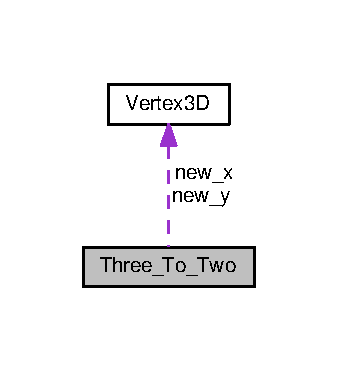
\includegraphics[width=162pt]{class_three___to___two__coll__graph}
\end{center}
\end{figure}
\subsection*{Public Member Functions}
\begin{DoxyCompactItemize}
\item 
void \hyperlink{class_three___to___two_ab3a3cda1a3f0e61b927c87e0a9655de6}{get\+Input} (string in)
\item 
void \hyperlink{class_three___to___two_a879354b0418511bd700d3f19c3cf8cbc}{set\+Plane} (float \hyperlink{draw2_8cpp_ad36c8f7a507294aa8f53bb0baf28fb24}{a1}, float \hyperlink{draw2_8cpp_a0a909289ec9fbfaa70c0e112ec9e3b15}{b1}, float \hyperlink{draw2_8cpp_a7fea4d2f6f3c31b60301494b136558af}{c1})
\item 
void \hyperlink{class_three___to___two_a00c909f873cde40038e9e077f9349162}{get\+Plane} ()
\item 
void \hyperlink{class_three___to___two_afcfa094efbefe5fc2c68129f0019328c}{shift\+\_\+origin} (bool calculate, bool \hyperlink{draw2_8cpp_ac5c54df7ed3b930268c8d7752c101725}{update})
\item 
void \hyperlink{class_three___to___two_aa783af2e5ff93ec80cb54bd9d70596ce}{scale} (float factor, bool autoscale, bool \hyperlink{draw2_8cpp_ac5c54df7ed3b930268c8d7752c101725}{update})
\item 
void \hyperlink{class_three___to___two_a741076f262ae512cca81ecff5f6f6b3b}{rotate\+\_\+axis} ()
\item 
void \hyperlink{class_three___to___two_ac3b4d37a5184425e327ff0ec0754ced6}{calc\+\_\+angle} ()
\item 
void \hyperlink{class_three___to___two_aee13f1c088479d2c414da9cbb25d7c65}{project} ()
\item 
bool \hyperlink{class_three___to___two_aa0a2e58b081bb7079b094c0b8ab974cc}{find\+In\+Vector} (vector$<$ \hyperlink{struct_vertex2_d}{Vertex2D} $>$ vec, \hyperlink{struct_vertex2_d}{Vertex2D} v)
\item 
void \hyperlink{class_three___to___two_a4b6515193b0bf2798ef792c0fc2998f4}{write\+Output} (string out)
\item 
void \hyperlink{class_three___to___two_ab630fa931ae0d5f46da926ad18e831f6}{plot\+Output} (string out)
\end{DoxyCompactItemize}
\subsection*{Public Attributes}
\begin{DoxyCompactItemize}
\item 
map$<$ string, vector$<$ \hyperlink{struct_vertex2_d}{Vertex2D} $>$ $>$ \hyperlink{class_three___to___two_a39ed690740565f107b2b65a678e0ab5e}{projection}
\item 
map$<$ string, list$<$ \hyperlink{struct_vertex3_d}{Vertex3D} $>$ $>$ \hyperlink{class_three___to___two_ab89e25f994881aea2bdae437e397f970}{model}
\item 
map$<$ string, string $>$ \hyperlink{class_three___to___two_a10db4a5f7a04743b00ce1f9215147dcc}{point\+To\+Proj}
\item 
map$<$ string, vector$<$ \hyperlink{struct_vertex3_d}{Vertex3D} $>$ $>$ \hyperlink{class_three___to___two_abb86c66855183ae0463c28af722997bb}{proj\+Labels}
\item 
map$<$ string, vector$<$ string $>$ $>$ \hyperlink{class_three___to___two_a2f86f24e2cbd6f19b7288c3b0f401f49}{faces\+\_\+vertices}
\item 
map$<$ string, vector$<$ string $>$ $>$ \hyperlink{class_three___to___two_ab76600933c530c9a6e7a54cf39df7bc9}{vertices\+\_\+faces}
\item 
float \hyperlink{class_three___to___two_a62f60abbec70c062d40369bae26d8bfc}{x} = 0.\+0
\item 
float \hyperlink{class_three___to___two_a74c72941752a52a87c13e4268ec37cc8}{y} = 0.\+0
\item 
float \hyperlink{class_three___to___two_a2dc98edd9d60378c346b61e988f966f9}{z} = 0.\+0
\item 
float \hyperlink{class_three___to___two_a8396aaabde6a54cdc6a36b6d263d94e5}{a} = 1.\+0
\item 
float \hyperlink{class_three___to___two_a4859d8dc45f60e772c55ab2923bab71c}{b} = 0.\+0
\item 
float \hyperlink{class_three___to___two_aaf40e46b50333549d03205a22974fce0}{c} = 0.\+0
\item 
int \hyperlink{class_three___to___two_abfb1f1c097808c8faf3f6cb28911491d}{choice} =0
\item 
\hyperlink{struct_vertex3_d}{Vertex3D} \hyperlink{class_three___to___two_a5e20357c42384b2e7aecfdf88ccbd898}{new\+\_\+x}
\item 
\hyperlink{struct_vertex3_d}{Vertex3D} \hyperlink{class_three___to___two_a6d516a8a5fa8b8ee2dd1c64195725ab7}{new\+\_\+y}
\item 
string \hyperlink{class_three___to___two_acdd6380173d6df1ce3d72c911ba0f1af}{input\+\_\+file}
\item 
string \hyperlink{class_three___to___two_a94c401d2acc198ffb188d37e7ce424c4}{output\+\_\+file}
\item 
map$<$ string, \hyperlink{struct_vertex3_d}{Vertex3D} $>$ \hyperlink{class_three___to___two_a2550b425f64bae1a0f92f5405dab24b2}{vertices}
\item 
map$<$ string, \hyperlink{struct_vertex2_d}{Vertex2D} $>$ \hyperlink{class_three___to___two_a579ed77ab975e6cfb1cf90d28074a93b}{result}
\item 
map$<$ pair$<$ float, float $>$, vector$<$ string $>$ $>$ \hyperlink{class_three___to___two_a1116965a6138a9b16fee724eccff6ba5}{vertices2D}
\item 
int \hyperlink{class_three___to___two_a9e131241a48170afd8af54e30ee95ded}{m} =0
\item 
int \hyperlink{class_three___to___two_a42a8bb1919cbeaa1a717ecea05468493}{n\+\_\+edges} =0
\item 
int \hyperlink{class_three___to___two_aef5084fad08c5eeac58437d90113122f}{n\+\_\+faces} =0
\item 
map$<$ string, string $>$ \hyperlink{class_three___to___two_a98ab641ba7f2da5fffbe0066debcafaa}{correspond}
\item 
vector$<$ pair$<$ string, string $>$ $>$ \hyperlink{class_three___to___two_aafa5fc739b2313e58a440d9b8b3d4875}{edges}
\item 
int \hyperlink{class_three___to___two_a3893134e478349a3df093541bc35f406}{n} = 0
\item 
float \hyperlink{class_three___to___two_a6e2169c85306e089975e4be179ab8869}{scale\+\_\+factor} = 1
\item 
vector$<$ string $>$ \hyperlink{class_three___to___two_a08809b4ff50badda240d9adb8847405c}{vertices\+\_\+list}
\item 
float \hyperlink{class_three___to___two_a6a7cf88c8d654edd486bc979284c256a}{alpha} = 0.\+0
\item 
float \hyperlink{class_three___to___two_a36bafd8c3cf8db0e6ea4f6f936922e3d}{beta} = 0.\+0
\item 
float \hyperlink{class_three___to___two_aefe3e71b2a022c70407771625a5b416e}{gamma} = 0.\+0
\end{DoxyCompactItemize}


\subsection{Detailed Description}


Definition at line 12 of file Three\+To\+Two.\+cpp.



\subsection{Member Function Documentation}
\index{Three\+\_\+\+To\+\_\+\+Two@{Three\+\_\+\+To\+\_\+\+Two}!calc\+\_\+angle@{calc\+\_\+angle}}
\index{calc\+\_\+angle@{calc\+\_\+angle}!Three\+\_\+\+To\+\_\+\+Two@{Three\+\_\+\+To\+\_\+\+Two}}
\subsubsection[{\texorpdfstring{calc\+\_\+angle()}{calc_angle()}}]{\setlength{\rightskip}{0pt plus 5cm}void Three\+\_\+\+To\+\_\+\+Two\+::calc\+\_\+angle (
\begin{DoxyParamCaption}
{}
\end{DoxyParamCaption}
)\hspace{0.3cm}{\ttfamily [inline]}}\hypertarget{class_three___to___two_ac3b4d37a5184425e327ff0ec0754ced6}{}\label{class_three___to___two_ac3b4d37a5184425e327ff0ec0754ced6}


Definition at line 414 of file Three\+To\+Two.\+cpp.

\index{Three\+\_\+\+To\+\_\+\+Two@{Three\+\_\+\+To\+\_\+\+Two}!find\+In\+Vector@{find\+In\+Vector}}
\index{find\+In\+Vector@{find\+In\+Vector}!Three\+\_\+\+To\+\_\+\+Two@{Three\+\_\+\+To\+\_\+\+Two}}
\subsubsection[{\texorpdfstring{find\+In\+Vector(vector$<$ Vertex2\+D $>$ vec, Vertex2\+D v)}{findInVector(vector< Vertex2D > vec, Vertex2D v)}}]{\setlength{\rightskip}{0pt plus 5cm}bool Three\+\_\+\+To\+\_\+\+Two\+::find\+In\+Vector (
\begin{DoxyParamCaption}
\item[{vector$<$ {\bf Vertex2D} $>$}]{vec, }
\item[{{\bf Vertex2D}}]{v}
\end{DoxyParamCaption}
)\hspace{0.3cm}{\ttfamily [inline]}}\hypertarget{class_three___to___two_aa0a2e58b081bb7079b094c0b8ab974cc}{}\label{class_three___to___two_aa0a2e58b081bb7079b094c0b8ab974cc}


Definition at line 550 of file Three\+To\+Two.\+cpp.

\index{Three\+\_\+\+To\+\_\+\+Two@{Three\+\_\+\+To\+\_\+\+Two}!get\+Input@{get\+Input}}
\index{get\+Input@{get\+Input}!Three\+\_\+\+To\+\_\+\+Two@{Three\+\_\+\+To\+\_\+\+Two}}
\subsubsection[{\texorpdfstring{get\+Input(string in)}{getInput(string in)}}]{\setlength{\rightskip}{0pt plus 5cm}void Three\+\_\+\+To\+\_\+\+Two\+::get\+Input (
\begin{DoxyParamCaption}
\item[{string}]{in}
\end{DoxyParamCaption}
)\hspace{0.3cm}{\ttfamily [inline]}}\hypertarget{class_three___to___two_ab3a3cda1a3f0e61b927c87e0a9655de6}{}\label{class_three___to___two_ab3a3cda1a3f0e61b927c87e0a9655de6}


Definition at line 69 of file Three\+To\+Two.\+cpp.

\index{Three\+\_\+\+To\+\_\+\+Two@{Three\+\_\+\+To\+\_\+\+Two}!get\+Plane@{get\+Plane}}
\index{get\+Plane@{get\+Plane}!Three\+\_\+\+To\+\_\+\+Two@{Three\+\_\+\+To\+\_\+\+Two}}
\subsubsection[{\texorpdfstring{get\+Plane()}{getPlane()}}]{\setlength{\rightskip}{0pt plus 5cm}void Three\+\_\+\+To\+\_\+\+Two\+::get\+Plane (
\begin{DoxyParamCaption}
{}
\end{DoxyParamCaption}
)\hspace{0.3cm}{\ttfamily [inline]}}\hypertarget{class_three___to___two_a00c909f873cde40038e9e077f9349162}{}\label{class_three___to___two_a00c909f873cde40038e9e077f9349162}


Definition at line 188 of file Three\+To\+Two.\+cpp.

\index{Three\+\_\+\+To\+\_\+\+Two@{Three\+\_\+\+To\+\_\+\+Two}!plot\+Output@{plot\+Output}}
\index{plot\+Output@{plot\+Output}!Three\+\_\+\+To\+\_\+\+Two@{Three\+\_\+\+To\+\_\+\+Two}}
\subsubsection[{\texorpdfstring{plot\+Output(string out)}{plotOutput(string out)}}]{\setlength{\rightskip}{0pt plus 5cm}void Three\+\_\+\+To\+\_\+\+Two\+::plot\+Output (
\begin{DoxyParamCaption}
\item[{string}]{out}
\end{DoxyParamCaption}
)\hspace{0.3cm}{\ttfamily [inline]}}\hypertarget{class_three___to___two_ab630fa931ae0d5f46da926ad18e831f6}{}\label{class_three___to___two_ab630fa931ae0d5f46da926ad18e831f6}


Definition at line 601 of file Three\+To\+Two.\+cpp.

\index{Three\+\_\+\+To\+\_\+\+Two@{Three\+\_\+\+To\+\_\+\+Two}!project@{project}}
\index{project@{project}!Three\+\_\+\+To\+\_\+\+Two@{Three\+\_\+\+To\+\_\+\+Two}}
\subsubsection[{\texorpdfstring{project()}{project()}}]{\setlength{\rightskip}{0pt plus 5cm}void Three\+\_\+\+To\+\_\+\+Two\+::project (
\begin{DoxyParamCaption}
{}
\end{DoxyParamCaption}
)\hspace{0.3cm}{\ttfamily [inline]}}\hypertarget{class_three___to___two_aee13f1c088479d2c414da9cbb25d7c65}{}\label{class_three___to___two_aee13f1c088479d2c414da9cbb25d7c65}


Definition at line 425 of file Three\+To\+Two.\+cpp.

\index{Three\+\_\+\+To\+\_\+\+Two@{Three\+\_\+\+To\+\_\+\+Two}!rotate\+\_\+axis@{rotate\+\_\+axis}}
\index{rotate\+\_\+axis@{rotate\+\_\+axis}!Three\+\_\+\+To\+\_\+\+Two@{Three\+\_\+\+To\+\_\+\+Two}}
\subsubsection[{\texorpdfstring{rotate\+\_\+axis()}{rotate_axis()}}]{\setlength{\rightskip}{0pt plus 5cm}void Three\+\_\+\+To\+\_\+\+Two\+::rotate\+\_\+axis (
\begin{DoxyParamCaption}
{}
\end{DoxyParamCaption}
)\hspace{0.3cm}{\ttfamily [inline]}}\hypertarget{class_three___to___two_a741076f262ae512cca81ecff5f6f6b3b}{}\label{class_three___to___two_a741076f262ae512cca81ecff5f6f6b3b}


Definition at line 363 of file Three\+To\+Two.\+cpp.

\index{Three\+\_\+\+To\+\_\+\+Two@{Three\+\_\+\+To\+\_\+\+Two}!scale@{scale}}
\index{scale@{scale}!Three\+\_\+\+To\+\_\+\+Two@{Three\+\_\+\+To\+\_\+\+Two}}
\subsubsection[{\texorpdfstring{scale(float factor, bool autoscale, bool update)}{scale(float factor, bool autoscale, bool update)}}]{\setlength{\rightskip}{0pt plus 5cm}void Three\+\_\+\+To\+\_\+\+Two\+::scale (
\begin{DoxyParamCaption}
\item[{float}]{factor, }
\item[{bool}]{autoscale, }
\item[{bool}]{update}
\end{DoxyParamCaption}
)\hspace{0.3cm}{\ttfamily [inline]}}\hypertarget{class_three___to___two_aa783af2e5ff93ec80cb54bd9d70596ce}{}\label{class_three___to___two_aa783af2e5ff93ec80cb54bd9d70596ce}


Definition at line 302 of file Three\+To\+Two.\+cpp.

\index{Three\+\_\+\+To\+\_\+\+Two@{Three\+\_\+\+To\+\_\+\+Two}!set\+Plane@{set\+Plane}}
\index{set\+Plane@{set\+Plane}!Three\+\_\+\+To\+\_\+\+Two@{Three\+\_\+\+To\+\_\+\+Two}}
\subsubsection[{\texorpdfstring{set\+Plane(float a1, float b1, float c1)}{setPlane(float a1, float b1, float c1)}}]{\setlength{\rightskip}{0pt plus 5cm}void Three\+\_\+\+To\+\_\+\+Two\+::set\+Plane (
\begin{DoxyParamCaption}
\item[{float}]{a1, }
\item[{float}]{b1, }
\item[{float}]{c1}
\end{DoxyParamCaption}
)\hspace{0.3cm}{\ttfamily [inline]}}\hypertarget{class_three___to___two_a879354b0418511bd700d3f19c3cf8cbc}{}\label{class_three___to___two_a879354b0418511bd700d3f19c3cf8cbc}


Definition at line 181 of file Three\+To\+Two.\+cpp.

\index{Three\+\_\+\+To\+\_\+\+Two@{Three\+\_\+\+To\+\_\+\+Two}!shift\+\_\+origin@{shift\+\_\+origin}}
\index{shift\+\_\+origin@{shift\+\_\+origin}!Three\+\_\+\+To\+\_\+\+Two@{Three\+\_\+\+To\+\_\+\+Two}}
\subsubsection[{\texorpdfstring{shift\+\_\+origin(bool calculate, bool update)}{shift_origin(bool calculate, bool update)}}]{\setlength{\rightskip}{0pt plus 5cm}void Three\+\_\+\+To\+\_\+\+Two\+::shift\+\_\+origin (
\begin{DoxyParamCaption}
\item[{bool}]{calculate, }
\item[{bool}]{update}
\end{DoxyParamCaption}
)\hspace{0.3cm}{\ttfamily [inline]}}\hypertarget{class_three___to___two_afcfa094efbefe5fc2c68129f0019328c}{}\label{class_three___to___two_afcfa094efbefe5fc2c68129f0019328c}


Definition at line 250 of file Three\+To\+Two.\+cpp.

\index{Three\+\_\+\+To\+\_\+\+Two@{Three\+\_\+\+To\+\_\+\+Two}!write\+Output@{write\+Output}}
\index{write\+Output@{write\+Output}!Three\+\_\+\+To\+\_\+\+Two@{Three\+\_\+\+To\+\_\+\+Two}}
\subsubsection[{\texorpdfstring{write\+Output(string out)}{writeOutput(string out)}}]{\setlength{\rightskip}{0pt plus 5cm}void Three\+\_\+\+To\+\_\+\+Two\+::write\+Output (
\begin{DoxyParamCaption}
\item[{string}]{out}
\end{DoxyParamCaption}
)\hspace{0.3cm}{\ttfamily [inline]}}\hypertarget{class_three___to___two_a4b6515193b0bf2798ef792c0fc2998f4}{}\label{class_three___to___two_a4b6515193b0bf2798ef792c0fc2998f4}


Definition at line 560 of file Three\+To\+Two.\+cpp.



\subsection{Member Data Documentation}
\index{Three\+\_\+\+To\+\_\+\+Two@{Three\+\_\+\+To\+\_\+\+Two}!a@{a}}
\index{a@{a}!Three\+\_\+\+To\+\_\+\+Two@{Three\+\_\+\+To\+\_\+\+Two}}
\subsubsection[{\texorpdfstring{a}{a}}]{\setlength{\rightskip}{0pt plus 5cm}float Three\+\_\+\+To\+\_\+\+Two\+::a = 1.\+0}\hypertarget{class_three___to___two_a8396aaabde6a54cdc6a36b6d263d94e5}{}\label{class_three___to___two_a8396aaabde6a54cdc6a36b6d263d94e5}


Definition at line 34 of file Three\+To\+Two.\+cpp.

\index{Three\+\_\+\+To\+\_\+\+Two@{Three\+\_\+\+To\+\_\+\+Two}!alpha@{alpha}}
\index{alpha@{alpha}!Three\+\_\+\+To\+\_\+\+Two@{Three\+\_\+\+To\+\_\+\+Two}}
\subsubsection[{\texorpdfstring{alpha}{alpha}}]{\setlength{\rightskip}{0pt plus 5cm}float Three\+\_\+\+To\+\_\+\+Two\+::alpha = 0.\+0}\hypertarget{class_three___to___two_a6a7cf88c8d654edd486bc979284c256a}{}\label{class_three___to___two_a6a7cf88c8d654edd486bc979284c256a}


Definition at line 66 of file Three\+To\+Two.\+cpp.

\index{Three\+\_\+\+To\+\_\+\+Two@{Three\+\_\+\+To\+\_\+\+Two}!b@{b}}
\index{b@{b}!Three\+\_\+\+To\+\_\+\+Two@{Three\+\_\+\+To\+\_\+\+Two}}
\subsubsection[{\texorpdfstring{b}{b}}]{\setlength{\rightskip}{0pt plus 5cm}float Three\+\_\+\+To\+\_\+\+Two\+::b = 0.\+0}\hypertarget{class_three___to___two_a4859d8dc45f60e772c55ab2923bab71c}{}\label{class_three___to___two_a4859d8dc45f60e772c55ab2923bab71c}


Definition at line 35 of file Three\+To\+Two.\+cpp.

\index{Three\+\_\+\+To\+\_\+\+Two@{Three\+\_\+\+To\+\_\+\+Two}!beta@{beta}}
\index{beta@{beta}!Three\+\_\+\+To\+\_\+\+Two@{Three\+\_\+\+To\+\_\+\+Two}}
\subsubsection[{\texorpdfstring{beta}{beta}}]{\setlength{\rightskip}{0pt plus 5cm}float Three\+\_\+\+To\+\_\+\+Two\+::beta = 0.\+0}\hypertarget{class_three___to___two_a36bafd8c3cf8db0e6ea4f6f936922e3d}{}\label{class_three___to___two_a36bafd8c3cf8db0e6ea4f6f936922e3d}


Definition at line 66 of file Three\+To\+Two.\+cpp.

\index{Three\+\_\+\+To\+\_\+\+Two@{Three\+\_\+\+To\+\_\+\+Two}!c@{c}}
\index{c@{c}!Three\+\_\+\+To\+\_\+\+Two@{Three\+\_\+\+To\+\_\+\+Two}}
\subsubsection[{\texorpdfstring{c}{c}}]{\setlength{\rightskip}{0pt plus 5cm}float Three\+\_\+\+To\+\_\+\+Two\+::c = 0.\+0}\hypertarget{class_three___to___two_aaf40e46b50333549d03205a22974fce0}{}\label{class_three___to___two_aaf40e46b50333549d03205a22974fce0}


Definition at line 36 of file Three\+To\+Two.\+cpp.

\index{Three\+\_\+\+To\+\_\+\+Two@{Three\+\_\+\+To\+\_\+\+Two}!choice@{choice}}
\index{choice@{choice}!Three\+\_\+\+To\+\_\+\+Two@{Three\+\_\+\+To\+\_\+\+Two}}
\subsubsection[{\texorpdfstring{choice}{choice}}]{\setlength{\rightskip}{0pt plus 5cm}int Three\+\_\+\+To\+\_\+\+Two\+::choice =0}\hypertarget{class_three___to___two_abfb1f1c097808c8faf3f6cb28911491d}{}\label{class_three___to___two_abfb1f1c097808c8faf3f6cb28911491d}


Definition at line 38 of file Three\+To\+Two.\+cpp.

\index{Three\+\_\+\+To\+\_\+\+Two@{Three\+\_\+\+To\+\_\+\+Two}!correspond@{correspond}}
\index{correspond@{correspond}!Three\+\_\+\+To\+\_\+\+Two@{Three\+\_\+\+To\+\_\+\+Two}}
\subsubsection[{\texorpdfstring{correspond}{correspond}}]{\setlength{\rightskip}{0pt plus 5cm}map$<$string,string$>$ Three\+\_\+\+To\+\_\+\+Two\+::correspond}\hypertarget{class_three___to___two_a98ab641ba7f2da5fffbe0066debcafaa}{}\label{class_three___to___two_a98ab641ba7f2da5fffbe0066debcafaa}


Definition at line 55 of file Three\+To\+Two.\+cpp.

\index{Three\+\_\+\+To\+\_\+\+Two@{Three\+\_\+\+To\+\_\+\+Two}!edges@{edges}}
\index{edges@{edges}!Three\+\_\+\+To\+\_\+\+Two@{Three\+\_\+\+To\+\_\+\+Two}}
\subsubsection[{\texorpdfstring{edges}{edges}}]{\setlength{\rightskip}{0pt plus 5cm}vector$<$pair$<$string,string$>$ $>$ Three\+\_\+\+To\+\_\+\+Two\+::edges}\hypertarget{class_three___to___two_aafa5fc739b2313e58a440d9b8b3d4875}{}\label{class_three___to___two_aafa5fc739b2313e58a440d9b8b3d4875}


Definition at line 58 of file Three\+To\+Two.\+cpp.

\index{Three\+\_\+\+To\+\_\+\+Two@{Three\+\_\+\+To\+\_\+\+Two}!faces\+\_\+vertices@{faces\+\_\+vertices}}
\index{faces\+\_\+vertices@{faces\+\_\+vertices}!Three\+\_\+\+To\+\_\+\+Two@{Three\+\_\+\+To\+\_\+\+Two}}
\subsubsection[{\texorpdfstring{faces\+\_\+vertices}{faces_vertices}}]{\setlength{\rightskip}{0pt plus 5cm}map$<$ string, vector$<$string$>$ $>$ Three\+\_\+\+To\+\_\+\+Two\+::faces\+\_\+vertices}\hypertarget{class_three___to___two_a2f86f24e2cbd6f19b7288c3b0f401f49}{}\label{class_three___to___two_a2f86f24e2cbd6f19b7288c3b0f401f49}


Definition at line 28 of file Three\+To\+Two.\+cpp.

\index{Three\+\_\+\+To\+\_\+\+Two@{Three\+\_\+\+To\+\_\+\+Two}!gamma@{gamma}}
\index{gamma@{gamma}!Three\+\_\+\+To\+\_\+\+Two@{Three\+\_\+\+To\+\_\+\+Two}}
\subsubsection[{\texorpdfstring{gamma}{gamma}}]{\setlength{\rightskip}{0pt plus 5cm}float Three\+\_\+\+To\+\_\+\+Two\+::gamma = 0.\+0}\hypertarget{class_three___to___two_aefe3e71b2a022c70407771625a5b416e}{}\label{class_three___to___two_aefe3e71b2a022c70407771625a5b416e}


Definition at line 66 of file Three\+To\+Two.\+cpp.

\index{Three\+\_\+\+To\+\_\+\+Two@{Three\+\_\+\+To\+\_\+\+Two}!input\+\_\+file@{input\+\_\+file}}
\index{input\+\_\+file@{input\+\_\+file}!Three\+\_\+\+To\+\_\+\+Two@{Three\+\_\+\+To\+\_\+\+Two}}
\subsubsection[{\texorpdfstring{input\+\_\+file}{input_file}}]{\setlength{\rightskip}{0pt plus 5cm}string Three\+\_\+\+To\+\_\+\+Two\+::input\+\_\+file}\hypertarget{class_three___to___two_acdd6380173d6df1ce3d72c911ba0f1af}{}\label{class_three___to___two_acdd6380173d6df1ce3d72c911ba0f1af}


Definition at line 43 of file Three\+To\+Two.\+cpp.

\index{Three\+\_\+\+To\+\_\+\+Two@{Three\+\_\+\+To\+\_\+\+Two}!m@{m}}
\index{m@{m}!Three\+\_\+\+To\+\_\+\+Two@{Three\+\_\+\+To\+\_\+\+Two}}
\subsubsection[{\texorpdfstring{m}{m}}]{\setlength{\rightskip}{0pt plus 5cm}int Three\+\_\+\+To\+\_\+\+Two\+::m =0}\hypertarget{class_three___to___two_a9e131241a48170afd8af54e30ee95ded}{}\label{class_three___to___two_a9e131241a48170afd8af54e30ee95ded}


Definition at line 53 of file Three\+To\+Two.\+cpp.

\index{Three\+\_\+\+To\+\_\+\+Two@{Three\+\_\+\+To\+\_\+\+Two}!model@{model}}
\index{model@{model}!Three\+\_\+\+To\+\_\+\+Two@{Three\+\_\+\+To\+\_\+\+Two}}
\subsubsection[{\texorpdfstring{model}{model}}]{\setlength{\rightskip}{0pt plus 5cm}map$<$string, list$<${\bf Vertex3D}$>$ $>$ Three\+\_\+\+To\+\_\+\+Two\+::model}\hypertarget{class_three___to___two_ab89e25f994881aea2bdae437e397f970}{}\label{class_three___to___two_ab89e25f994881aea2bdae437e397f970}


Definition at line 19 of file Three\+To\+Two.\+cpp.

\index{Three\+\_\+\+To\+\_\+\+Two@{Three\+\_\+\+To\+\_\+\+Two}!n@{n}}
\index{n@{n}!Three\+\_\+\+To\+\_\+\+Two@{Three\+\_\+\+To\+\_\+\+Two}}
\subsubsection[{\texorpdfstring{n}{n}}]{\setlength{\rightskip}{0pt plus 5cm}int Three\+\_\+\+To\+\_\+\+Two\+::n = 0}\hypertarget{class_three___to___two_a3893134e478349a3df093541bc35f406}{}\label{class_three___to___two_a3893134e478349a3df093541bc35f406}


Definition at line 60 of file Three\+To\+Two.\+cpp.

\index{Three\+\_\+\+To\+\_\+\+Two@{Three\+\_\+\+To\+\_\+\+Two}!n\+\_\+edges@{n\+\_\+edges}}
\index{n\+\_\+edges@{n\+\_\+edges}!Three\+\_\+\+To\+\_\+\+Two@{Three\+\_\+\+To\+\_\+\+Two}}
\subsubsection[{\texorpdfstring{n\+\_\+edges}{n_edges}}]{\setlength{\rightskip}{0pt plus 5cm}int Three\+\_\+\+To\+\_\+\+Two\+::n\+\_\+edges =0}\hypertarget{class_three___to___two_a42a8bb1919cbeaa1a717ecea05468493}{}\label{class_three___to___two_a42a8bb1919cbeaa1a717ecea05468493}


Definition at line 53 of file Three\+To\+Two.\+cpp.

\index{Three\+\_\+\+To\+\_\+\+Two@{Three\+\_\+\+To\+\_\+\+Two}!n\+\_\+faces@{n\+\_\+faces}}
\index{n\+\_\+faces@{n\+\_\+faces}!Three\+\_\+\+To\+\_\+\+Two@{Three\+\_\+\+To\+\_\+\+Two}}
\subsubsection[{\texorpdfstring{n\+\_\+faces}{n_faces}}]{\setlength{\rightskip}{0pt plus 5cm}int Three\+\_\+\+To\+\_\+\+Two\+::n\+\_\+faces =0}\hypertarget{class_three___to___two_aef5084fad08c5eeac58437d90113122f}{}\label{class_three___to___two_aef5084fad08c5eeac58437d90113122f}


Definition at line 53 of file Three\+To\+Two.\+cpp.

\index{Three\+\_\+\+To\+\_\+\+Two@{Three\+\_\+\+To\+\_\+\+Two}!new\+\_\+x@{new\+\_\+x}}
\index{new\+\_\+x@{new\+\_\+x}!Three\+\_\+\+To\+\_\+\+Two@{Three\+\_\+\+To\+\_\+\+Two}}
\subsubsection[{\texorpdfstring{new\+\_\+x}{new_x}}]{\setlength{\rightskip}{0pt plus 5cm}{\bf Vertex3D} Three\+\_\+\+To\+\_\+\+Two\+::new\+\_\+x}\hypertarget{class_three___to___two_a5e20357c42384b2e7aecfdf88ccbd898}{}\label{class_three___to___two_a5e20357c42384b2e7aecfdf88ccbd898}


Definition at line 40 of file Three\+To\+Two.\+cpp.

\index{Three\+\_\+\+To\+\_\+\+Two@{Three\+\_\+\+To\+\_\+\+Two}!new\+\_\+y@{new\+\_\+y}}
\index{new\+\_\+y@{new\+\_\+y}!Three\+\_\+\+To\+\_\+\+Two@{Three\+\_\+\+To\+\_\+\+Two}}
\subsubsection[{\texorpdfstring{new\+\_\+y}{new_y}}]{\setlength{\rightskip}{0pt plus 5cm}{\bf Vertex3D} Three\+\_\+\+To\+\_\+\+Two\+::new\+\_\+y}\hypertarget{class_three___to___two_a6d516a8a5fa8b8ee2dd1c64195725ab7}{}\label{class_three___to___two_a6d516a8a5fa8b8ee2dd1c64195725ab7}


Definition at line 40 of file Three\+To\+Two.\+cpp.

\index{Three\+\_\+\+To\+\_\+\+Two@{Three\+\_\+\+To\+\_\+\+Two}!output\+\_\+file@{output\+\_\+file}}
\index{output\+\_\+file@{output\+\_\+file}!Three\+\_\+\+To\+\_\+\+Two@{Three\+\_\+\+To\+\_\+\+Two}}
\subsubsection[{\texorpdfstring{output\+\_\+file}{output_file}}]{\setlength{\rightskip}{0pt plus 5cm}string Three\+\_\+\+To\+\_\+\+Two\+::output\+\_\+file}\hypertarget{class_three___to___two_a94c401d2acc198ffb188d37e7ce424c4}{}\label{class_three___to___two_a94c401d2acc198ffb188d37e7ce424c4}


Definition at line 44 of file Three\+To\+Two.\+cpp.

\index{Three\+\_\+\+To\+\_\+\+Two@{Three\+\_\+\+To\+\_\+\+Two}!point\+To\+Proj@{point\+To\+Proj}}
\index{point\+To\+Proj@{point\+To\+Proj}!Three\+\_\+\+To\+\_\+\+Two@{Three\+\_\+\+To\+\_\+\+Two}}
\subsubsection[{\texorpdfstring{point\+To\+Proj}{pointToProj}}]{\setlength{\rightskip}{0pt plus 5cm}map$<$ string, string$>$ Three\+\_\+\+To\+\_\+\+Two\+::point\+To\+Proj}\hypertarget{class_three___to___two_a10db4a5f7a04743b00ce1f9215147dcc}{}\label{class_three___to___two_a10db4a5f7a04743b00ce1f9215147dcc}


Definition at line 22 of file Three\+To\+Two.\+cpp.

\index{Three\+\_\+\+To\+\_\+\+Two@{Three\+\_\+\+To\+\_\+\+Two}!projection@{projection}}
\index{projection@{projection}!Three\+\_\+\+To\+\_\+\+Two@{Three\+\_\+\+To\+\_\+\+Two}}
\subsubsection[{\texorpdfstring{projection}{projection}}]{\setlength{\rightskip}{0pt plus 5cm}map$<$string, vector$<${\bf Vertex2D}$>$ $>$ Three\+\_\+\+To\+\_\+\+Two\+::projection}\hypertarget{class_three___to___two_a39ed690740565f107b2b65a678e0ab5e}{}\label{class_three___to___two_a39ed690740565f107b2b65a678e0ab5e}


Definition at line 17 of file Three\+To\+Two.\+cpp.

\index{Three\+\_\+\+To\+\_\+\+Two@{Three\+\_\+\+To\+\_\+\+Two}!proj\+Labels@{proj\+Labels}}
\index{proj\+Labels@{proj\+Labels}!Three\+\_\+\+To\+\_\+\+Two@{Three\+\_\+\+To\+\_\+\+Two}}
\subsubsection[{\texorpdfstring{proj\+Labels}{projLabels}}]{\setlength{\rightskip}{0pt plus 5cm}map$<$ string, vector$<${\bf Vertex3D}$>$ $>$ Three\+\_\+\+To\+\_\+\+Two\+::proj\+Labels}\hypertarget{class_three___to___two_abb86c66855183ae0463c28af722997bb}{}\label{class_three___to___two_abb86c66855183ae0463c28af722997bb}


Definition at line 25 of file Three\+To\+Two.\+cpp.

\index{Three\+\_\+\+To\+\_\+\+Two@{Three\+\_\+\+To\+\_\+\+Two}!result@{result}}
\index{result@{result}!Three\+\_\+\+To\+\_\+\+Two@{Three\+\_\+\+To\+\_\+\+Two}}
\subsubsection[{\texorpdfstring{result}{result}}]{\setlength{\rightskip}{0pt plus 5cm}map$<$string, {\bf Vertex2D}$>$ Three\+\_\+\+To\+\_\+\+Two\+::result}\hypertarget{class_three___to___two_a579ed77ab975e6cfb1cf90d28074a93b}{}\label{class_three___to___two_a579ed77ab975e6cfb1cf90d28074a93b}


Definition at line 50 of file Three\+To\+Two.\+cpp.

\index{Three\+\_\+\+To\+\_\+\+Two@{Three\+\_\+\+To\+\_\+\+Two}!scale\+\_\+factor@{scale\+\_\+factor}}
\index{scale\+\_\+factor@{scale\+\_\+factor}!Three\+\_\+\+To\+\_\+\+Two@{Three\+\_\+\+To\+\_\+\+Two}}
\subsubsection[{\texorpdfstring{scale\+\_\+factor}{scale_factor}}]{\setlength{\rightskip}{0pt plus 5cm}float Three\+\_\+\+To\+\_\+\+Two\+::scale\+\_\+factor = 1}\hypertarget{class_three___to___two_a6e2169c85306e089975e4be179ab8869}{}\label{class_three___to___two_a6e2169c85306e089975e4be179ab8869}


Definition at line 61 of file Three\+To\+Two.\+cpp.

\index{Three\+\_\+\+To\+\_\+\+Two@{Three\+\_\+\+To\+\_\+\+Two}!vertices@{vertices}}
\index{vertices@{vertices}!Three\+\_\+\+To\+\_\+\+Two@{Three\+\_\+\+To\+\_\+\+Two}}
\subsubsection[{\texorpdfstring{vertices}{vertices}}]{\setlength{\rightskip}{0pt plus 5cm}map$<$string, {\bf Vertex3D}$>$ Three\+\_\+\+To\+\_\+\+Two\+::vertices}\hypertarget{class_three___to___two_a2550b425f64bae1a0f92f5405dab24b2}{}\label{class_three___to___two_a2550b425f64bae1a0f92f5405dab24b2}


Definition at line 47 of file Three\+To\+Two.\+cpp.

\index{Three\+\_\+\+To\+\_\+\+Two@{Three\+\_\+\+To\+\_\+\+Two}!vertices2D@{vertices2D}}
\index{vertices2D@{vertices2D}!Three\+\_\+\+To\+\_\+\+Two@{Three\+\_\+\+To\+\_\+\+Two}}
\subsubsection[{\texorpdfstring{vertices2D}{vertices2D}}]{\setlength{\rightskip}{0pt plus 5cm}map$<$pair$<$float,float$>$, vector$<$string$>$ $>$ Three\+\_\+\+To\+\_\+\+Two\+::vertices2D}\hypertarget{class_three___to___two_a1116965a6138a9b16fee724eccff6ba5}{}\label{class_three___to___two_a1116965a6138a9b16fee724eccff6ba5}


Definition at line 52 of file Three\+To\+Two.\+cpp.

\index{Three\+\_\+\+To\+\_\+\+Two@{Three\+\_\+\+To\+\_\+\+Two}!vertices\+\_\+faces@{vertices\+\_\+faces}}
\index{vertices\+\_\+faces@{vertices\+\_\+faces}!Three\+\_\+\+To\+\_\+\+Two@{Three\+\_\+\+To\+\_\+\+Two}}
\subsubsection[{\texorpdfstring{vertices\+\_\+faces}{vertices_faces}}]{\setlength{\rightskip}{0pt plus 5cm}map$<$ string, vector$<$string$>$ $>$ Three\+\_\+\+To\+\_\+\+Two\+::vertices\+\_\+faces}\hypertarget{class_three___to___two_ab76600933c530c9a6e7a54cf39df7bc9}{}\label{class_three___to___two_ab76600933c530c9a6e7a54cf39df7bc9}


Definition at line 31 of file Three\+To\+Two.\+cpp.

\index{Three\+\_\+\+To\+\_\+\+Two@{Three\+\_\+\+To\+\_\+\+Two}!vertices\+\_\+list@{vertices\+\_\+list}}
\index{vertices\+\_\+list@{vertices\+\_\+list}!Three\+\_\+\+To\+\_\+\+Two@{Three\+\_\+\+To\+\_\+\+Two}}
\subsubsection[{\texorpdfstring{vertices\+\_\+list}{vertices_list}}]{\setlength{\rightskip}{0pt plus 5cm}vector$<$string$>$ Three\+\_\+\+To\+\_\+\+Two\+::vertices\+\_\+list}\hypertarget{class_three___to___two_a08809b4ff50badda240d9adb8847405c}{}\label{class_three___to___two_a08809b4ff50badda240d9adb8847405c}


Definition at line 64 of file Three\+To\+Two.\+cpp.

\index{Three\+\_\+\+To\+\_\+\+Two@{Three\+\_\+\+To\+\_\+\+Two}!x@{x}}
\index{x@{x}!Three\+\_\+\+To\+\_\+\+Two@{Three\+\_\+\+To\+\_\+\+Two}}
\subsubsection[{\texorpdfstring{x}{x}}]{\setlength{\rightskip}{0pt plus 5cm}float Three\+\_\+\+To\+\_\+\+Two\+::x = 0.\+0}\hypertarget{class_three___to___two_a62f60abbec70c062d40369bae26d8bfc}{}\label{class_three___to___two_a62f60abbec70c062d40369bae26d8bfc}


Definition at line 33 of file Three\+To\+Two.\+cpp.

\index{Three\+\_\+\+To\+\_\+\+Two@{Three\+\_\+\+To\+\_\+\+Two}!y@{y}}
\index{y@{y}!Three\+\_\+\+To\+\_\+\+Two@{Three\+\_\+\+To\+\_\+\+Two}}
\subsubsection[{\texorpdfstring{y}{y}}]{\setlength{\rightskip}{0pt plus 5cm}float Three\+\_\+\+To\+\_\+\+Two\+::y = 0.\+0}\hypertarget{class_three___to___two_a74c72941752a52a87c13e4268ec37cc8}{}\label{class_three___to___two_a74c72941752a52a87c13e4268ec37cc8}


Definition at line 33 of file Three\+To\+Two.\+cpp.

\index{Three\+\_\+\+To\+\_\+\+Two@{Three\+\_\+\+To\+\_\+\+Two}!z@{z}}
\index{z@{z}!Three\+\_\+\+To\+\_\+\+Two@{Three\+\_\+\+To\+\_\+\+Two}}
\subsubsection[{\texorpdfstring{z}{z}}]{\setlength{\rightskip}{0pt plus 5cm}float Three\+\_\+\+To\+\_\+\+Two\+::z = 0.\+0}\hypertarget{class_three___to___two_a2dc98edd9d60378c346b61e988f966f9}{}\label{class_three___to___two_a2dc98edd9d60378c346b61e988f966f9}


Definition at line 33 of file Three\+To\+Two.\+cpp.



The documentation for this class was generated from the following file\+:\begin{DoxyCompactItemize}
\item 
src/\hyperlink{_three_to_two_8cpp}{Three\+To\+Two.\+cpp}\end{DoxyCompactItemize}

\hypertarget{class_two___to___three}{}\section{Two\+\_\+\+To\+\_\+\+Three Class Reference}
\label{class_two___to___three}\index{Two\+\_\+\+To\+\_\+\+Three@{Two\+\_\+\+To\+\_\+\+Three}}
\subsection*{Public Member Functions}
\begin{DoxyCompactItemize}
\item 
void \hyperlink{class_two___to___three_a8cb0750fd7f06f63f7c3959832d14b50}{get\+Input} (string xy, string yz, string zx)
\item 
void \hyperlink{class_two___to___three_a573db0749ff0865895c0ee59b11af430}{expand\+\_\+h} (vector$<$ pair$<$ string, string $>$$>$ \&edge\+\_\+xy1, map$<$ string, vector$<$ string $>$ $>$ \&rev\+\_\+xy1, vector$<$ pair$<$ string, string $>$$>$ \&exp\+\_\+xy1)
\item 
void \hyperlink{class_two___to___three_a33d7852f618104a0580629062bdb23df}{expand} ()
\item 
void \hyperlink{class_two___to___three_af04b2b2c81700169a740b7527f4fab5b}{eliminate\+\_\+h} (vector$<$ pair$<$ string, string $>$$>$ \&exp\+\_\+xy1, vector$<$ pair$<$ string, string $>$$>$ \&exp\+\_\+xy2, map$<$ string, string $>$ map\+\_\+xy2)
\item 
void \hyperlink{class_two___to___three_a8699e9b6b281e00271e1368ef088b14d}{eliminate} ()
\item 
void \hyperlink{class_two___to___three_a9dbc9fdd8e73ae2e3a974a624a33a6b0}{find\+\_\+all} ()
\item 
void \hyperlink{class_two___to___three_ad3a0d8e135d0dc58386e0055c70fe105}{edges\+\_\+one} (vector$<$ pair$<$ string, string $>$$>$ \&exp\+\_\+xy1)
\item 
void \hyperlink{class_two___to___three_a1b181eea2c5309d5264f27a7bb055168}{edges\+\_\+all} ()
\item 
void \hyperlink{class_two___to___three_af29125458d6479842f70e4a6c3fd0301}{write\+Output} (string out)
\item 
void \hyperlink{class_two___to___three_a3638cd9c0c945fa6eec51b890cb5a73b}{plot\+Output} (string out)
\end{DoxyCompactItemize}
\subsection*{Public Attributes}
\begin{DoxyCompactItemize}
\item 
string \hyperlink{class_two___to___three_a552bbac302db3a8d39d0b0c9014e717d}{xy\+\_\+file}
\item 
string \hyperlink{class_two___to___three_a17e155076c64e9207f9e10d7db944fbe}{yz\+\_\+file}
\item 
string \hyperlink{class_two___to___three_a102a4276583a481691dd6f717a81e11e}{zx\+\_\+file}
\item 
map$<$ string, \hyperlink{struct_vertex3_d}{Vertex3D} $>$ \hyperlink{class_two___to___three_aa57efe556b563e0e5b45fa9f1653c1cd}{model}
\item 
set$<$ string $>$ \hyperlink{class_two___to___three_a2f42478bfa5c2e759df2caac98e12b22}{vertices\+\_\+list}
\item 
map$<$ string, \hyperlink{struct_vertex2_d}{Vertex2D} $>$ \hyperlink{class_two___to___three_aa324b095f53b74973a1ed45d80bf401f}{vertices\+\_\+xy}
\item 
map$<$ string, \hyperlink{struct_vertex2_d}{Vertex2D} $>$ \hyperlink{class_two___to___three_a8052b332b93963257e5e1eff1acbf3f7}{vertices\+\_\+yz}
\item 
map$<$ string, \hyperlink{struct_vertex2_d}{Vertex2D} $>$ \hyperlink{class_two___to___three_a4bd1e4471ca424af9640f70f6b146fb1}{vertices\+\_\+zx}
\item 
map$<$ string, string $>$ \hyperlink{class_two___to___three_a699e1b081ba68063b84ee0628f1824f1}{map\+\_\+xy}
\item 
map$<$ string, string $>$ \hyperlink{class_two___to___three_ab50e85aa8226e964ba2fcbf95fade23d}{map\+\_\+yz}
\item 
map$<$ string, string $>$ \hyperlink{class_two___to___three_a6c016590ff5c2c305eaa571e6d8f47ed}{map\+\_\+zx}
\item 
vector$<$ pair$<$ string, string $>$ $>$ \hyperlink{class_two___to___three_aa0701d423859854d6dcf6a3948c3c797}{edge\+\_\+xy}
\item 
vector$<$ pair$<$ string, string $>$ $>$ \hyperlink{class_two___to___three_a8fa25ea9719f9ecea3d8a521f5e7e14c}{edge\+\_\+yz}
\item 
vector$<$ pair$<$ string, string $>$ $>$ \hyperlink{class_two___to___three_a1a77bc05b0101d52a3cdeca1cda97382}{edge\+\_\+zx}
\item 
vector$<$ pair$<$ string, string $>$ $>$ \hyperlink{class_two___to___three_a0fb51cd40a43e0371a930ecc7ae5cca7}{exp\+\_\+xy}
\item 
vector$<$ pair$<$ string, string $>$ $>$ \hyperlink{class_two___to___three_a2fd53fedb88911745fdfe403fe954194}{exp\+\_\+yz}
\item 
vector$<$ pair$<$ string, string $>$ $>$ \hyperlink{class_two___to___three_a0fc9541c8e1dc603ace96c135851ad26}{exp\+\_\+zx}
\item 
map$<$ string, vector$<$ string $>$ $>$ \hyperlink{class_two___to___three_a485336245fad21fd41d8552df9fe9dd1}{rev\+\_\+xy}
\item 
map$<$ string, vector$<$ string $>$ $>$ \hyperlink{class_two___to___three_afb85013e1ee6676f359de1f5c9e0a5da}{rev\+\_\+yz}
\item 
map$<$ string, vector$<$ string $>$ $>$ \hyperlink{class_two___to___three_a11ca3157f2afc24a1d896bd8a8232156}{rev\+\_\+zx}
\item 
set$<$ pair$<$ string, string $>$ $>$ \hyperlink{class_two___to___three_a1dea63027222bee8934b66010b0e44a3}{edges}
\item 
float \hyperlink{class_two___to___three_a388e406a03a64b5422f1de36c138ecaa}{scale\+\_\+factor} = 1
\end{DoxyCompactItemize}


\subsection{Detailed Description}


Definition at line 11 of file Two\+To\+Three.\+cpp.



\subsection{Member Function Documentation}
\index{Two\+\_\+\+To\+\_\+\+Three@{Two\+\_\+\+To\+\_\+\+Three}!edges\+\_\+all@{edges\+\_\+all}}
\index{edges\+\_\+all@{edges\+\_\+all}!Two\+\_\+\+To\+\_\+\+Three@{Two\+\_\+\+To\+\_\+\+Three}}
\subsubsection[{\texorpdfstring{edges\+\_\+all()}{edges_all()}}]{\setlength{\rightskip}{0pt plus 5cm}void Two\+\_\+\+To\+\_\+\+Three\+::edges\+\_\+all (
\begin{DoxyParamCaption}
{}
\end{DoxyParamCaption}
)\hspace{0.3cm}{\ttfamily [inline]}}\hypertarget{class_two___to___three_a1b181eea2c5309d5264f27a7bb055168}{}\label{class_two___to___three_a1b181eea2c5309d5264f27a7bb055168}


Definition at line 386 of file Two\+To\+Three.\+cpp.

\index{Two\+\_\+\+To\+\_\+\+Three@{Two\+\_\+\+To\+\_\+\+Three}!edges\+\_\+one@{edges\+\_\+one}}
\index{edges\+\_\+one@{edges\+\_\+one}!Two\+\_\+\+To\+\_\+\+Three@{Two\+\_\+\+To\+\_\+\+Three}}
\subsubsection[{\texorpdfstring{edges\+\_\+one(vector$<$ pair$<$ string, string $>$$>$ \&exp\+\_\+xy1)}{edges_one(vector< pair< string, string >> &exp_xy1)}}]{\setlength{\rightskip}{0pt plus 5cm}void Two\+\_\+\+To\+\_\+\+Three\+::edges\+\_\+one (
\begin{DoxyParamCaption}
\item[{vector$<$ pair$<$ string, string $>$$>$ \&}]{exp\+\_\+xy1}
\end{DoxyParamCaption}
)\hspace{0.3cm}{\ttfamily [inline]}}\hypertarget{class_two___to___three_ad3a0d8e135d0dc58386e0055c70fe105}{}\label{class_two___to___three_ad3a0d8e135d0dc58386e0055c70fe105}


Definition at line 376 of file Two\+To\+Three.\+cpp.

\index{Two\+\_\+\+To\+\_\+\+Three@{Two\+\_\+\+To\+\_\+\+Three}!eliminate@{eliminate}}
\index{eliminate@{eliminate}!Two\+\_\+\+To\+\_\+\+Three@{Two\+\_\+\+To\+\_\+\+Three}}
\subsubsection[{\texorpdfstring{eliminate()}{eliminate()}}]{\setlength{\rightskip}{0pt plus 5cm}void Two\+\_\+\+To\+\_\+\+Three\+::eliminate (
\begin{DoxyParamCaption}
{}
\end{DoxyParamCaption}
)\hspace{0.3cm}{\ttfamily [inline]}}\hypertarget{class_two___to___three_a8699e9b6b281e00271e1368ef088b14d}{}\label{class_two___to___three_a8699e9b6b281e00271e1368ef088b14d}


Definition at line 301 of file Two\+To\+Three.\+cpp.

\index{Two\+\_\+\+To\+\_\+\+Three@{Two\+\_\+\+To\+\_\+\+Three}!eliminate\+\_\+h@{eliminate\+\_\+h}}
\index{eliminate\+\_\+h@{eliminate\+\_\+h}!Two\+\_\+\+To\+\_\+\+Three@{Two\+\_\+\+To\+\_\+\+Three}}
\subsubsection[{\texorpdfstring{eliminate\+\_\+h(vector$<$ pair$<$ string, string $>$$>$ \&exp\+\_\+xy1, vector$<$ pair$<$ string, string $>$$>$ \&exp\+\_\+xy2, map$<$ string, string $>$ map\+\_\+xy2)}{eliminate_h(vector< pair< string, string >> &exp_xy1, vector< pair< string, string >> &exp_xy2, map< string, string > map_xy2)}}]{\setlength{\rightskip}{0pt plus 5cm}void Two\+\_\+\+To\+\_\+\+Three\+::eliminate\+\_\+h (
\begin{DoxyParamCaption}
\item[{vector$<$ pair$<$ string, string $>$$>$ \&}]{exp\+\_\+xy1, }
\item[{vector$<$ pair$<$ string, string $>$$>$ \&}]{exp\+\_\+xy2, }
\item[{map$<$ string, string $>$}]{map\+\_\+xy2}
\end{DoxyParamCaption}
)\hspace{0.3cm}{\ttfamily [inline]}}\hypertarget{class_two___to___three_af04b2b2c81700169a740b7527f4fab5b}{}\label{class_two___to___three_af04b2b2c81700169a740b7527f4fab5b}


Definition at line 260 of file Two\+To\+Three.\+cpp.

\index{Two\+\_\+\+To\+\_\+\+Three@{Two\+\_\+\+To\+\_\+\+Three}!expand@{expand}}
\index{expand@{expand}!Two\+\_\+\+To\+\_\+\+Three@{Two\+\_\+\+To\+\_\+\+Three}}
\subsubsection[{\texorpdfstring{expand()}{expand()}}]{\setlength{\rightskip}{0pt plus 5cm}void Two\+\_\+\+To\+\_\+\+Three\+::expand (
\begin{DoxyParamCaption}
{}
\end{DoxyParamCaption}
)\hspace{0.3cm}{\ttfamily [inline]}}\hypertarget{class_two___to___three_a33d7852f618104a0580629062bdb23df}{}\label{class_two___to___three_a33d7852f618104a0580629062bdb23df}


Definition at line 250 of file Two\+To\+Three.\+cpp.

\index{Two\+\_\+\+To\+\_\+\+Three@{Two\+\_\+\+To\+\_\+\+Three}!expand\+\_\+h@{expand\+\_\+h}}
\index{expand\+\_\+h@{expand\+\_\+h}!Two\+\_\+\+To\+\_\+\+Three@{Two\+\_\+\+To\+\_\+\+Three}}
\subsubsection[{\texorpdfstring{expand\+\_\+h(vector$<$ pair$<$ string, string $>$$>$ \&edge\+\_\+xy1, map$<$ string, vector$<$ string $>$ $>$ \&rev\+\_\+xy1, vector$<$ pair$<$ string, string $>$$>$ \&exp\+\_\+xy1)}{expand_h(vector< pair< string, string >> &edge_xy1, map< string, vector< string > > &rev_xy1, vector< pair< string, string >> &exp_xy1)}}]{\setlength{\rightskip}{0pt plus 5cm}void Two\+\_\+\+To\+\_\+\+Three\+::expand\+\_\+h (
\begin{DoxyParamCaption}
\item[{vector$<$ pair$<$ string, string $>$$>$ \&}]{edge\+\_\+xy1, }
\item[{map$<$ string, vector$<$ string $>$ $>$ \&}]{rev\+\_\+xy1, }
\item[{vector$<$ pair$<$ string, string $>$$>$ \&}]{exp\+\_\+xy1}
\end{DoxyParamCaption}
)\hspace{0.3cm}{\ttfamily [inline]}}\hypertarget{class_two___to___three_a573db0749ff0865895c0ee59b11af430}{}\label{class_two___to___three_a573db0749ff0865895c0ee59b11af430}


Definition at line 222 of file Two\+To\+Three.\+cpp.

\index{Two\+\_\+\+To\+\_\+\+Three@{Two\+\_\+\+To\+\_\+\+Three}!find\+\_\+all@{find\+\_\+all}}
\index{find\+\_\+all@{find\+\_\+all}!Two\+\_\+\+To\+\_\+\+Three@{Two\+\_\+\+To\+\_\+\+Three}}
\subsubsection[{\texorpdfstring{find\+\_\+all()}{find_all()}}]{\setlength{\rightskip}{0pt plus 5cm}void Two\+\_\+\+To\+\_\+\+Three\+::find\+\_\+all (
\begin{DoxyParamCaption}
{}
\end{DoxyParamCaption}
)\hspace{0.3cm}{\ttfamily [inline]}}\hypertarget{class_two___to___three_a9dbc9fdd8e73ae2e3a974a624a33a6b0}{}\label{class_two___to___three_a9dbc9fdd8e73ae2e3a974a624a33a6b0}


Definition at line 315 of file Two\+To\+Three.\+cpp.

\index{Two\+\_\+\+To\+\_\+\+Three@{Two\+\_\+\+To\+\_\+\+Three}!get\+Input@{get\+Input}}
\index{get\+Input@{get\+Input}!Two\+\_\+\+To\+\_\+\+Three@{Two\+\_\+\+To\+\_\+\+Three}}
\subsubsection[{\texorpdfstring{get\+Input(string xy, string yz, string zx)}{getInput(string xy, string yz, string zx)}}]{\setlength{\rightskip}{0pt plus 5cm}void Two\+\_\+\+To\+\_\+\+Three\+::get\+Input (
\begin{DoxyParamCaption}
\item[{string}]{xy, }
\item[{string}]{yz, }
\item[{string}]{zx}
\end{DoxyParamCaption}
)\hspace{0.3cm}{\ttfamily [inline]}}\hypertarget{class_two___to___three_a8cb0750fd7f06f63f7c3959832d14b50}{}\label{class_two___to___three_a8cb0750fd7f06f63f7c3959832d14b50}


Definition at line 56 of file Two\+To\+Three.\+cpp.

\index{Two\+\_\+\+To\+\_\+\+Three@{Two\+\_\+\+To\+\_\+\+Three}!plot\+Output@{plot\+Output}}
\index{plot\+Output@{plot\+Output}!Two\+\_\+\+To\+\_\+\+Three@{Two\+\_\+\+To\+\_\+\+Three}}
\subsubsection[{\texorpdfstring{plot\+Output(string out)}{plotOutput(string out)}}]{\setlength{\rightskip}{0pt plus 5cm}void Two\+\_\+\+To\+\_\+\+Three\+::plot\+Output (
\begin{DoxyParamCaption}
\item[{string}]{out}
\end{DoxyParamCaption}
)\hspace{0.3cm}{\ttfamily [inline]}}\hypertarget{class_two___to___three_a3638cd9c0c945fa6eec51b890cb5a73b}{}\label{class_two___to___three_a3638cd9c0c945fa6eec51b890cb5a73b}


Definition at line 431 of file Two\+To\+Three.\+cpp.

\index{Two\+\_\+\+To\+\_\+\+Three@{Two\+\_\+\+To\+\_\+\+Three}!write\+Output@{write\+Output}}
\index{write\+Output@{write\+Output}!Two\+\_\+\+To\+\_\+\+Three@{Two\+\_\+\+To\+\_\+\+Three}}
\subsubsection[{\texorpdfstring{write\+Output(string out)}{writeOutput(string out)}}]{\setlength{\rightskip}{0pt plus 5cm}void Two\+\_\+\+To\+\_\+\+Three\+::write\+Output (
\begin{DoxyParamCaption}
\item[{string}]{out}
\end{DoxyParamCaption}
)\hspace{0.3cm}{\ttfamily [inline]}}\hypertarget{class_two___to___three_af29125458d6479842f70e4a6c3fd0301}{}\label{class_two___to___three_af29125458d6479842f70e4a6c3fd0301}


Definition at line 395 of file Two\+To\+Three.\+cpp.



\subsection{Member Data Documentation}
\index{Two\+\_\+\+To\+\_\+\+Three@{Two\+\_\+\+To\+\_\+\+Three}!edge\+\_\+xy@{edge\+\_\+xy}}
\index{edge\+\_\+xy@{edge\+\_\+xy}!Two\+\_\+\+To\+\_\+\+Three@{Two\+\_\+\+To\+\_\+\+Three}}
\subsubsection[{\texorpdfstring{edge\+\_\+xy}{edge_xy}}]{\setlength{\rightskip}{0pt plus 5cm}vector$<$pair$<$string,string$>$ $>$ Two\+\_\+\+To\+\_\+\+Three\+::edge\+\_\+xy}\hypertarget{class_two___to___three_aa0701d423859854d6dcf6a3948c3c797}{}\label{class_two___to___three_aa0701d423859854d6dcf6a3948c3c797}


Definition at line 34 of file Two\+To\+Three.\+cpp.

\index{Two\+\_\+\+To\+\_\+\+Three@{Two\+\_\+\+To\+\_\+\+Three}!edge\+\_\+yz@{edge\+\_\+yz}}
\index{edge\+\_\+yz@{edge\+\_\+yz}!Two\+\_\+\+To\+\_\+\+Three@{Two\+\_\+\+To\+\_\+\+Three}}
\subsubsection[{\texorpdfstring{edge\+\_\+yz}{edge_yz}}]{\setlength{\rightskip}{0pt plus 5cm}vector$<$pair$<$string,string$>$ $>$ Two\+\_\+\+To\+\_\+\+Three\+::edge\+\_\+yz}\hypertarget{class_two___to___three_a8fa25ea9719f9ecea3d8a521f5e7e14c}{}\label{class_two___to___three_a8fa25ea9719f9ecea3d8a521f5e7e14c}


Definition at line 35 of file Two\+To\+Three.\+cpp.

\index{Two\+\_\+\+To\+\_\+\+Three@{Two\+\_\+\+To\+\_\+\+Three}!edge\+\_\+zx@{edge\+\_\+zx}}
\index{edge\+\_\+zx@{edge\+\_\+zx}!Two\+\_\+\+To\+\_\+\+Three@{Two\+\_\+\+To\+\_\+\+Three}}
\subsubsection[{\texorpdfstring{edge\+\_\+zx}{edge_zx}}]{\setlength{\rightskip}{0pt plus 5cm}vector$<$pair$<$string,string$>$ $>$ Two\+\_\+\+To\+\_\+\+Three\+::edge\+\_\+zx}\hypertarget{class_two___to___three_a1a77bc05b0101d52a3cdeca1cda97382}{}\label{class_two___to___three_a1a77bc05b0101d52a3cdeca1cda97382}


Definition at line 36 of file Two\+To\+Three.\+cpp.

\index{Two\+\_\+\+To\+\_\+\+Three@{Two\+\_\+\+To\+\_\+\+Three}!edges@{edges}}
\index{edges@{edges}!Two\+\_\+\+To\+\_\+\+Three@{Two\+\_\+\+To\+\_\+\+Three}}
\subsubsection[{\texorpdfstring{edges}{edges}}]{\setlength{\rightskip}{0pt plus 5cm}set$<$pair$<$string,string$>$ $>$ Two\+\_\+\+To\+\_\+\+Three\+::edges}\hypertarget{class_two___to___three_a1dea63027222bee8934b66010b0e44a3}{}\label{class_two___to___three_a1dea63027222bee8934b66010b0e44a3}


Definition at line 49 of file Two\+To\+Three.\+cpp.

\index{Two\+\_\+\+To\+\_\+\+Three@{Two\+\_\+\+To\+\_\+\+Three}!exp\+\_\+xy@{exp\+\_\+xy}}
\index{exp\+\_\+xy@{exp\+\_\+xy}!Two\+\_\+\+To\+\_\+\+Three@{Two\+\_\+\+To\+\_\+\+Three}}
\subsubsection[{\texorpdfstring{exp\+\_\+xy}{exp_xy}}]{\setlength{\rightskip}{0pt plus 5cm}vector$<$pair$<$string,string$>$ $>$ Two\+\_\+\+To\+\_\+\+Three\+::exp\+\_\+xy}\hypertarget{class_two___to___three_a0fb51cd40a43e0371a930ecc7ae5cca7}{}\label{class_two___to___three_a0fb51cd40a43e0371a930ecc7ae5cca7}


Definition at line 39 of file Two\+To\+Three.\+cpp.

\index{Two\+\_\+\+To\+\_\+\+Three@{Two\+\_\+\+To\+\_\+\+Three}!exp\+\_\+yz@{exp\+\_\+yz}}
\index{exp\+\_\+yz@{exp\+\_\+yz}!Two\+\_\+\+To\+\_\+\+Three@{Two\+\_\+\+To\+\_\+\+Three}}
\subsubsection[{\texorpdfstring{exp\+\_\+yz}{exp_yz}}]{\setlength{\rightskip}{0pt plus 5cm}vector$<$pair$<$string,string$>$ $>$ Two\+\_\+\+To\+\_\+\+Three\+::exp\+\_\+yz}\hypertarget{class_two___to___three_a2fd53fedb88911745fdfe403fe954194}{}\label{class_two___to___three_a2fd53fedb88911745fdfe403fe954194}


Definition at line 40 of file Two\+To\+Three.\+cpp.

\index{Two\+\_\+\+To\+\_\+\+Three@{Two\+\_\+\+To\+\_\+\+Three}!exp\+\_\+zx@{exp\+\_\+zx}}
\index{exp\+\_\+zx@{exp\+\_\+zx}!Two\+\_\+\+To\+\_\+\+Three@{Two\+\_\+\+To\+\_\+\+Three}}
\subsubsection[{\texorpdfstring{exp\+\_\+zx}{exp_zx}}]{\setlength{\rightskip}{0pt plus 5cm}vector$<$pair$<$string,string$>$ $>$ Two\+\_\+\+To\+\_\+\+Three\+::exp\+\_\+zx}\hypertarget{class_two___to___three_a0fc9541c8e1dc603ace96c135851ad26}{}\label{class_two___to___three_a0fc9541c8e1dc603ace96c135851ad26}


Definition at line 41 of file Two\+To\+Three.\+cpp.

\index{Two\+\_\+\+To\+\_\+\+Three@{Two\+\_\+\+To\+\_\+\+Three}!map\+\_\+xy@{map\+\_\+xy}}
\index{map\+\_\+xy@{map\+\_\+xy}!Two\+\_\+\+To\+\_\+\+Three@{Two\+\_\+\+To\+\_\+\+Three}}
\subsubsection[{\texorpdfstring{map\+\_\+xy}{map_xy}}]{\setlength{\rightskip}{0pt plus 5cm}map$<$string, string$>$ Two\+\_\+\+To\+\_\+\+Three\+::map\+\_\+xy}\hypertarget{class_two___to___three_a699e1b081ba68063b84ee0628f1824f1}{}\label{class_two___to___three_a699e1b081ba68063b84ee0628f1824f1}


Definition at line 29 of file Two\+To\+Three.\+cpp.

\index{Two\+\_\+\+To\+\_\+\+Three@{Two\+\_\+\+To\+\_\+\+Three}!map\+\_\+yz@{map\+\_\+yz}}
\index{map\+\_\+yz@{map\+\_\+yz}!Two\+\_\+\+To\+\_\+\+Three@{Two\+\_\+\+To\+\_\+\+Three}}
\subsubsection[{\texorpdfstring{map\+\_\+yz}{map_yz}}]{\setlength{\rightskip}{0pt plus 5cm}map$<$string, string$>$ Two\+\_\+\+To\+\_\+\+Three\+::map\+\_\+yz}\hypertarget{class_two___to___three_ab50e85aa8226e964ba2fcbf95fade23d}{}\label{class_two___to___three_ab50e85aa8226e964ba2fcbf95fade23d}


Definition at line 30 of file Two\+To\+Three.\+cpp.

\index{Two\+\_\+\+To\+\_\+\+Three@{Two\+\_\+\+To\+\_\+\+Three}!map\+\_\+zx@{map\+\_\+zx}}
\index{map\+\_\+zx@{map\+\_\+zx}!Two\+\_\+\+To\+\_\+\+Three@{Two\+\_\+\+To\+\_\+\+Three}}
\subsubsection[{\texorpdfstring{map\+\_\+zx}{map_zx}}]{\setlength{\rightskip}{0pt plus 5cm}map$<$string, string$>$ Two\+\_\+\+To\+\_\+\+Three\+::map\+\_\+zx}\hypertarget{class_two___to___three_a6c016590ff5c2c305eaa571e6d8f47ed}{}\label{class_two___to___three_a6c016590ff5c2c305eaa571e6d8f47ed}


Definition at line 31 of file Two\+To\+Three.\+cpp.

\index{Two\+\_\+\+To\+\_\+\+Three@{Two\+\_\+\+To\+\_\+\+Three}!model@{model}}
\index{model@{model}!Two\+\_\+\+To\+\_\+\+Three@{Two\+\_\+\+To\+\_\+\+Three}}
\subsubsection[{\texorpdfstring{model}{model}}]{\setlength{\rightskip}{0pt plus 5cm}map$<$string, {\bf Vertex3D} $>$ Two\+\_\+\+To\+\_\+\+Three\+::model}\hypertarget{class_two___to___three_aa57efe556b563e0e5b45fa9f1653c1cd}{}\label{class_two___to___three_aa57efe556b563e0e5b45fa9f1653c1cd}


Definition at line 18 of file Two\+To\+Three.\+cpp.

\index{Two\+\_\+\+To\+\_\+\+Three@{Two\+\_\+\+To\+\_\+\+Three}!rev\+\_\+xy@{rev\+\_\+xy}}
\index{rev\+\_\+xy@{rev\+\_\+xy}!Two\+\_\+\+To\+\_\+\+Three@{Two\+\_\+\+To\+\_\+\+Three}}
\subsubsection[{\texorpdfstring{rev\+\_\+xy}{rev_xy}}]{\setlength{\rightskip}{0pt plus 5cm}map$<$string, vector$<$string$>$ $>$ Two\+\_\+\+To\+\_\+\+Three\+::rev\+\_\+xy}\hypertarget{class_two___to___three_a485336245fad21fd41d8552df9fe9dd1}{}\label{class_two___to___three_a485336245fad21fd41d8552df9fe9dd1}


Definition at line 44 of file Two\+To\+Three.\+cpp.

\index{Two\+\_\+\+To\+\_\+\+Three@{Two\+\_\+\+To\+\_\+\+Three}!rev\+\_\+yz@{rev\+\_\+yz}}
\index{rev\+\_\+yz@{rev\+\_\+yz}!Two\+\_\+\+To\+\_\+\+Three@{Two\+\_\+\+To\+\_\+\+Three}}
\subsubsection[{\texorpdfstring{rev\+\_\+yz}{rev_yz}}]{\setlength{\rightskip}{0pt plus 5cm}map$<$string, vector$<$string$>$ $>$ Two\+\_\+\+To\+\_\+\+Three\+::rev\+\_\+yz}\hypertarget{class_two___to___three_afb85013e1ee6676f359de1f5c9e0a5da}{}\label{class_two___to___three_afb85013e1ee6676f359de1f5c9e0a5da}


Definition at line 45 of file Two\+To\+Three.\+cpp.

\index{Two\+\_\+\+To\+\_\+\+Three@{Two\+\_\+\+To\+\_\+\+Three}!rev\+\_\+zx@{rev\+\_\+zx}}
\index{rev\+\_\+zx@{rev\+\_\+zx}!Two\+\_\+\+To\+\_\+\+Three@{Two\+\_\+\+To\+\_\+\+Three}}
\subsubsection[{\texorpdfstring{rev\+\_\+zx}{rev_zx}}]{\setlength{\rightskip}{0pt plus 5cm}map$<$string, vector$<$string$>$ $>$ Two\+\_\+\+To\+\_\+\+Three\+::rev\+\_\+zx}\hypertarget{class_two___to___three_a11ca3157f2afc24a1d896bd8a8232156}{}\label{class_two___to___three_a11ca3157f2afc24a1d896bd8a8232156}


Definition at line 46 of file Two\+To\+Three.\+cpp.

\index{Two\+\_\+\+To\+\_\+\+Three@{Two\+\_\+\+To\+\_\+\+Three}!scale\+\_\+factor@{scale\+\_\+factor}}
\index{scale\+\_\+factor@{scale\+\_\+factor}!Two\+\_\+\+To\+\_\+\+Three@{Two\+\_\+\+To\+\_\+\+Three}}
\subsubsection[{\texorpdfstring{scale\+\_\+factor}{scale_factor}}]{\setlength{\rightskip}{0pt plus 5cm}float Two\+\_\+\+To\+\_\+\+Three\+::scale\+\_\+factor = 1}\hypertarget{class_two___to___three_a388e406a03a64b5422f1de36c138ecaa}{}\label{class_two___to___three_a388e406a03a64b5422f1de36c138ecaa}


Definition at line 51 of file Two\+To\+Three.\+cpp.

\index{Two\+\_\+\+To\+\_\+\+Three@{Two\+\_\+\+To\+\_\+\+Three}!vertices\+\_\+list@{vertices\+\_\+list}}
\index{vertices\+\_\+list@{vertices\+\_\+list}!Two\+\_\+\+To\+\_\+\+Three@{Two\+\_\+\+To\+\_\+\+Three}}
\subsubsection[{\texorpdfstring{vertices\+\_\+list}{vertices_list}}]{\setlength{\rightskip}{0pt plus 5cm}set$<$string$>$ Two\+\_\+\+To\+\_\+\+Three\+::vertices\+\_\+list}\hypertarget{class_two___to___three_a2f42478bfa5c2e759df2caac98e12b22}{}\label{class_two___to___three_a2f42478bfa5c2e759df2caac98e12b22}


Definition at line 21 of file Two\+To\+Three.\+cpp.

\index{Two\+\_\+\+To\+\_\+\+Three@{Two\+\_\+\+To\+\_\+\+Three}!vertices\+\_\+xy@{vertices\+\_\+xy}}
\index{vertices\+\_\+xy@{vertices\+\_\+xy}!Two\+\_\+\+To\+\_\+\+Three@{Two\+\_\+\+To\+\_\+\+Three}}
\subsubsection[{\texorpdfstring{vertices\+\_\+xy}{vertices_xy}}]{\setlength{\rightskip}{0pt plus 5cm}map$<$string, {\bf Vertex2D}$>$ Two\+\_\+\+To\+\_\+\+Three\+::vertices\+\_\+xy}\hypertarget{class_two___to___three_aa324b095f53b74973a1ed45d80bf401f}{}\label{class_two___to___three_aa324b095f53b74973a1ed45d80bf401f}


Definition at line 24 of file Two\+To\+Three.\+cpp.

\index{Two\+\_\+\+To\+\_\+\+Three@{Two\+\_\+\+To\+\_\+\+Three}!vertices\+\_\+yz@{vertices\+\_\+yz}}
\index{vertices\+\_\+yz@{vertices\+\_\+yz}!Two\+\_\+\+To\+\_\+\+Three@{Two\+\_\+\+To\+\_\+\+Three}}
\subsubsection[{\texorpdfstring{vertices\+\_\+yz}{vertices_yz}}]{\setlength{\rightskip}{0pt plus 5cm}map$<$string, {\bf Vertex2D}$>$ Two\+\_\+\+To\+\_\+\+Three\+::vertices\+\_\+yz}\hypertarget{class_two___to___three_a8052b332b93963257e5e1eff1acbf3f7}{}\label{class_two___to___three_a8052b332b93963257e5e1eff1acbf3f7}


Definition at line 25 of file Two\+To\+Three.\+cpp.

\index{Two\+\_\+\+To\+\_\+\+Three@{Two\+\_\+\+To\+\_\+\+Three}!vertices\+\_\+zx@{vertices\+\_\+zx}}
\index{vertices\+\_\+zx@{vertices\+\_\+zx}!Two\+\_\+\+To\+\_\+\+Three@{Two\+\_\+\+To\+\_\+\+Three}}
\subsubsection[{\texorpdfstring{vertices\+\_\+zx}{vertices_zx}}]{\setlength{\rightskip}{0pt plus 5cm}map$<$string, {\bf Vertex2D}$>$ Two\+\_\+\+To\+\_\+\+Three\+::vertices\+\_\+zx}\hypertarget{class_two___to___three_a4bd1e4471ca424af9640f70f6b146fb1}{}\label{class_two___to___three_a4bd1e4471ca424af9640f70f6b146fb1}


Definition at line 26 of file Two\+To\+Three.\+cpp.

\index{Two\+\_\+\+To\+\_\+\+Three@{Two\+\_\+\+To\+\_\+\+Three}!xy\+\_\+file@{xy\+\_\+file}}
\index{xy\+\_\+file@{xy\+\_\+file}!Two\+\_\+\+To\+\_\+\+Three@{Two\+\_\+\+To\+\_\+\+Three}}
\subsubsection[{\texorpdfstring{xy\+\_\+file}{xy_file}}]{\setlength{\rightskip}{0pt plus 5cm}string Two\+\_\+\+To\+\_\+\+Three\+::xy\+\_\+file}\hypertarget{class_two___to___three_a552bbac302db3a8d39d0b0c9014e717d}{}\label{class_two___to___three_a552bbac302db3a8d39d0b0c9014e717d}


Definition at line 15 of file Two\+To\+Three.\+cpp.

\index{Two\+\_\+\+To\+\_\+\+Three@{Two\+\_\+\+To\+\_\+\+Three}!yz\+\_\+file@{yz\+\_\+file}}
\index{yz\+\_\+file@{yz\+\_\+file}!Two\+\_\+\+To\+\_\+\+Three@{Two\+\_\+\+To\+\_\+\+Three}}
\subsubsection[{\texorpdfstring{yz\+\_\+file}{yz_file}}]{\setlength{\rightskip}{0pt plus 5cm}string Two\+\_\+\+To\+\_\+\+Three\+::yz\+\_\+file}\hypertarget{class_two___to___three_a17e155076c64e9207f9e10d7db944fbe}{}\label{class_two___to___three_a17e155076c64e9207f9e10d7db944fbe}


Definition at line 15 of file Two\+To\+Three.\+cpp.

\index{Two\+\_\+\+To\+\_\+\+Three@{Two\+\_\+\+To\+\_\+\+Three}!zx\+\_\+file@{zx\+\_\+file}}
\index{zx\+\_\+file@{zx\+\_\+file}!Two\+\_\+\+To\+\_\+\+Three@{Two\+\_\+\+To\+\_\+\+Three}}
\subsubsection[{\texorpdfstring{zx\+\_\+file}{zx_file}}]{\setlength{\rightskip}{0pt plus 5cm}string Two\+\_\+\+To\+\_\+\+Three\+::zx\+\_\+file}\hypertarget{class_two___to___three_a102a4276583a481691dd6f717a81e11e}{}\label{class_two___to___three_a102a4276583a481691dd6f717a81e11e}


Definition at line 15 of file Two\+To\+Three.\+cpp.



The documentation for this class was generated from the following file\+:\begin{DoxyCompactItemize}
\item 
src/\hyperlink{_two_to_three_8cpp}{Two\+To\+Three.\+cpp}\end{DoxyCompactItemize}

\hypertarget{structvertex2_d}{}\section{vertex2D Struct Reference}
\label{structvertex2_d}\index{vertex2D@{vertex2D}}


{\ttfamily \#include $<$structs.\+h$>$}

\subsection*{Public Attributes}
\begin{DoxyCompactItemize}
\item 
std\+::string \hyperlink{structvertex2_d_a92a0d499a4a4de12f7ea36423eb550b8}{label}
\item 
float \hyperlink{structvertex2_d_a2ba74d18c3e8e5a36fd2846a7a4d1a4f}{x}
\item 
float \hyperlink{structvertex2_d_a6ca32b6427f8d3ce3437db0bafd92a00}{y}
\end{DoxyCompactItemize}


\subsection{Detailed Description}


Definition at line 3 of file structs.\+h.



\subsection{Member Data Documentation}
\index{vertex2D@{vertex2D}!label@{label}}
\index{label@{label}!vertex2D@{vertex2D}}
\subsubsection[{\texorpdfstring{label}{label}}]{\setlength{\rightskip}{0pt plus 5cm}std\+::string vertex2\+D\+::label}\hypertarget{structvertex2_d_a92a0d499a4a4de12f7ea36423eb550b8}{}\label{structvertex2_d_a92a0d499a4a4de12f7ea36423eb550b8}


Definition at line 5 of file structs.\+h.

\index{vertex2D@{vertex2D}!x@{x}}
\index{x@{x}!vertex2D@{vertex2D}}
\subsubsection[{\texorpdfstring{x}{x}}]{\setlength{\rightskip}{0pt plus 5cm}float vertex2\+D\+::x}\hypertarget{structvertex2_d_a2ba74d18c3e8e5a36fd2846a7a4d1a4f}{}\label{structvertex2_d_a2ba74d18c3e8e5a36fd2846a7a4d1a4f}


Definition at line 6 of file structs.\+h.

\index{vertex2D@{vertex2D}!y@{y}}
\index{y@{y}!vertex2D@{vertex2D}}
\subsubsection[{\texorpdfstring{y}{y}}]{\setlength{\rightskip}{0pt plus 5cm}float vertex2\+D\+::y}\hypertarget{structvertex2_d_a6ca32b6427f8d3ce3437db0bafd92a00}{}\label{structvertex2_d_a6ca32b6427f8d3ce3437db0bafd92a00}


Definition at line 7 of file structs.\+h.



The documentation for this struct was generated from the following file\+:\begin{DoxyCompactItemize}
\item 
lib/\hyperlink{structs_8h}{structs.\+h}\end{DoxyCompactItemize}

\hypertarget{struct_vertex2_d}{}\section{Vertex2D Struct Reference}
\label{struct_vertex2_d}\index{Vertex2D@{Vertex2D}}
\subsection*{Public Attributes}
\begin{DoxyCompactItemize}
\item 
string \hyperlink{struct_vertex2_d_a549a8dbf41453045e1ffe05f0fd5e288}{label}
\item 
float \hyperlink{struct_vertex2_d_a39275a5945c972e573be08b52031a7d4}{x}
\item 
float \hyperlink{struct_vertex2_d_ac3948cfb8740e52bfa30daaf17cc5043}{y}
\end{DoxyCompactItemize}


\subsection{Detailed Description}


Definition at line 4 of file Vertex.\+cpp.



\subsection{Member Data Documentation}
\index{Vertex2D@{Vertex2D}!label@{label}}
\index{label@{label}!Vertex2D@{Vertex2D}}
\subsubsection[{\texorpdfstring{label}{label}}]{\setlength{\rightskip}{0pt plus 5cm}string Vertex2\+D\+::label}\hypertarget{struct_vertex2_d_a549a8dbf41453045e1ffe05f0fd5e288}{}\label{struct_vertex2_d_a549a8dbf41453045e1ffe05f0fd5e288}


Definition at line 6 of file Vertex.\+cpp.

\index{Vertex2D@{Vertex2D}!x@{x}}
\index{x@{x}!Vertex2D@{Vertex2D}}
\subsubsection[{\texorpdfstring{x}{x}}]{\setlength{\rightskip}{0pt plus 5cm}float Vertex2\+D\+::x}\hypertarget{struct_vertex2_d_a39275a5945c972e573be08b52031a7d4}{}\label{struct_vertex2_d_a39275a5945c972e573be08b52031a7d4}


Definition at line 7 of file Vertex.\+cpp.

\index{Vertex2D@{Vertex2D}!y@{y}}
\index{y@{y}!Vertex2D@{Vertex2D}}
\subsubsection[{\texorpdfstring{y}{y}}]{\setlength{\rightskip}{0pt plus 5cm}float Vertex2\+D\+::y}\hypertarget{struct_vertex2_d_ac3948cfb8740e52bfa30daaf17cc5043}{}\label{struct_vertex2_d_ac3948cfb8740e52bfa30daaf17cc5043}


Definition at line 8 of file Vertex.\+cpp.



The documentation for this struct was generated from the following file\+:\begin{DoxyCompactItemize}
\item 
lib/\hyperlink{_vertex_8cpp}{Vertex.\+cpp}\end{DoxyCompactItemize}

\hypertarget{structvertex3_d}{}\section{vertex3D Struct Reference}
\label{structvertex3_d}\index{vertex3D@{vertex3D}}


{\ttfamily \#include $<$structs.\+h$>$}

\subsection*{Public Attributes}
\begin{DoxyCompactItemize}
\item 
std\+::string \hyperlink{structvertex3_d_a6294e6614f1bb7ac73020c203a5f34c1}{label}
\item 
float \hyperlink{structvertex3_d_a6c6ee4315d72adbc5abb17e6af802087}{x}
\item 
float \hyperlink{structvertex3_d_aa1f4823bf2a3f648b1b0b39ef7ea5891}{y}
\item 
float \hyperlink{structvertex3_d_a67f3819dff895cb47284c34ec85658d7}{z}
\end{DoxyCompactItemize}


\subsection{Detailed Description}


Definition at line 10 of file structs.\+h.



\subsection{Member Data Documentation}
\index{vertex3D@{vertex3D}!label@{label}}
\index{label@{label}!vertex3D@{vertex3D}}
\subsubsection[{\texorpdfstring{label}{label}}]{\setlength{\rightskip}{0pt plus 5cm}std\+::string vertex3\+D\+::label}\hypertarget{structvertex3_d_a6294e6614f1bb7ac73020c203a5f34c1}{}\label{structvertex3_d_a6294e6614f1bb7ac73020c203a5f34c1}


Definition at line 12 of file structs.\+h.

\index{vertex3D@{vertex3D}!x@{x}}
\index{x@{x}!vertex3D@{vertex3D}}
\subsubsection[{\texorpdfstring{x}{x}}]{\setlength{\rightskip}{0pt plus 5cm}float vertex3\+D\+::x}\hypertarget{structvertex3_d_a6c6ee4315d72adbc5abb17e6af802087}{}\label{structvertex3_d_a6c6ee4315d72adbc5abb17e6af802087}


Definition at line 13 of file structs.\+h.

\index{vertex3D@{vertex3D}!y@{y}}
\index{y@{y}!vertex3D@{vertex3D}}
\subsubsection[{\texorpdfstring{y}{y}}]{\setlength{\rightskip}{0pt plus 5cm}float vertex3\+D\+::y}\hypertarget{structvertex3_d_aa1f4823bf2a3f648b1b0b39ef7ea5891}{}\label{structvertex3_d_aa1f4823bf2a3f648b1b0b39ef7ea5891}


Definition at line 14 of file structs.\+h.

\index{vertex3D@{vertex3D}!z@{z}}
\index{z@{z}!vertex3D@{vertex3D}}
\subsubsection[{\texorpdfstring{z}{z}}]{\setlength{\rightskip}{0pt plus 5cm}float vertex3\+D\+::z}\hypertarget{structvertex3_d_a67f3819dff895cb47284c34ec85658d7}{}\label{structvertex3_d_a67f3819dff895cb47284c34ec85658d7}


Definition at line 15 of file structs.\+h.



The documentation for this struct was generated from the following file\+:\begin{DoxyCompactItemize}
\item 
lib/\hyperlink{structs_8h}{structs.\+h}\end{DoxyCompactItemize}

\hypertarget{struct_vertex3_d}{}\section{Vertex3D Struct Reference}
\label{struct_vertex3_d}\index{Vertex3D@{Vertex3D}}
\subsection*{Public Attributes}
\begin{DoxyCompactItemize}
\item 
string \hyperlink{struct_vertex3_d_a4b0958099770a13662a0b4f95bccf4ff}{label}
\item 
float \hyperlink{struct_vertex3_d_a31874fac8de9ea8aa004f7d62c3b0a82}{x}
\item 
float \hyperlink{struct_vertex3_d_acc2ceb770e03d6facf4c921de0eaf3d8}{y}
\item 
float \hyperlink{struct_vertex3_d_af04a23eeeea792a53123e2d622395f8f}{z}
\item 
float \hyperlink{struct_vertex3_d_aba4baf3fd67dd3668a921b1030d089dd}{distance}
\end{DoxyCompactItemize}


\subsection{Detailed Description}


Definition at line 18 of file Vertex.\+cpp.



\subsection{Member Data Documentation}
\index{Vertex3D@{Vertex3D}!distance@{distance}}
\index{distance@{distance}!Vertex3D@{Vertex3D}}
\subsubsection[{\texorpdfstring{distance}{distance}}]{\setlength{\rightskip}{0pt plus 5cm}float Vertex3\+D\+::distance}\hypertarget{struct_vertex3_d_aba4baf3fd67dd3668a921b1030d089dd}{}\label{struct_vertex3_d_aba4baf3fd67dd3668a921b1030d089dd}


Definition at line 24 of file Vertex.\+cpp.

\index{Vertex3D@{Vertex3D}!label@{label}}
\index{label@{label}!Vertex3D@{Vertex3D}}
\subsubsection[{\texorpdfstring{label}{label}}]{\setlength{\rightskip}{0pt plus 5cm}string Vertex3\+D\+::label}\hypertarget{struct_vertex3_d_a4b0958099770a13662a0b4f95bccf4ff}{}\label{struct_vertex3_d_a4b0958099770a13662a0b4f95bccf4ff}


Definition at line 20 of file Vertex.\+cpp.

\index{Vertex3D@{Vertex3D}!x@{x}}
\index{x@{x}!Vertex3D@{Vertex3D}}
\subsubsection[{\texorpdfstring{x}{x}}]{\setlength{\rightskip}{0pt plus 5cm}float Vertex3\+D\+::x}\hypertarget{struct_vertex3_d_a31874fac8de9ea8aa004f7d62c3b0a82}{}\label{struct_vertex3_d_a31874fac8de9ea8aa004f7d62c3b0a82}


Definition at line 21 of file Vertex.\+cpp.

\index{Vertex3D@{Vertex3D}!y@{y}}
\index{y@{y}!Vertex3D@{Vertex3D}}
\subsubsection[{\texorpdfstring{y}{y}}]{\setlength{\rightskip}{0pt plus 5cm}float Vertex3\+D\+::y}\hypertarget{struct_vertex3_d_acc2ceb770e03d6facf4c921de0eaf3d8}{}\label{struct_vertex3_d_acc2ceb770e03d6facf4c921de0eaf3d8}


Definition at line 22 of file Vertex.\+cpp.

\index{Vertex3D@{Vertex3D}!z@{z}}
\index{z@{z}!Vertex3D@{Vertex3D}}
\subsubsection[{\texorpdfstring{z}{z}}]{\setlength{\rightskip}{0pt plus 5cm}float Vertex3\+D\+::z}\hypertarget{struct_vertex3_d_af04a23eeeea792a53123e2d622395f8f}{}\label{struct_vertex3_d_af04a23eeeea792a53123e2d622395f8f}


Definition at line 23 of file Vertex.\+cpp.



The documentation for this struct was generated from the following file\+:\begin{DoxyCompactItemize}
\item 
lib/\hyperlink{_vertex_8cpp}{Vertex.\+cpp}\end{DoxyCompactItemize}

\chapter{File Documentation}
\hypertarget{structs_8h}{}\section{lib/structs.h File Reference}
\label{structs_8h}\index{lib/structs.\+h@{lib/structs.\+h}}
{\ttfamily \#include $<$string$>$}\\*
Include dependency graph for structs.\+h\+:
\nopagebreak
\begin{figure}[H]
\begin{center}
\leavevmode
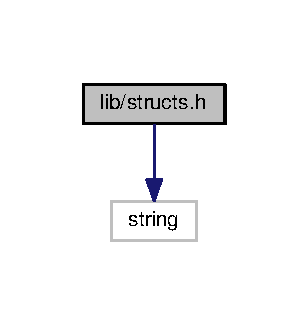
\includegraphics[width=148pt]{structs_8h__incl}
\end{center}
\end{figure}
\subsection*{Classes}
\begin{DoxyCompactItemize}
\item 
struct \hyperlink{structvertex2_d}{vertex2D}
\item 
struct \hyperlink{structvertex3_d}{vertex3D}
\end{DoxyCompactItemize}

\hypertarget{_vertex_8cpp}{}\section{lib/\+Vertex.cpp File Reference}
\label{_vertex_8cpp}\index{lib/\+Vertex.\+cpp@{lib/\+Vertex.\+cpp}}
{\ttfamily \#include $<$bits/stdc++.\+h$>$}\\*
Include dependency graph for Vertex.\+cpp\+:
\nopagebreak
\begin{figure}[H]
\begin{center}
\leavevmode
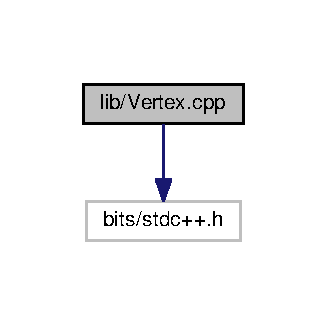
\includegraphics[width=157pt]{_vertex_8cpp__incl}
\end{center}
\end{figure}
This graph shows which files directly or indirectly include this file\+:
\nopagebreak
\begin{figure}[H]
\begin{center}
\leavevmode
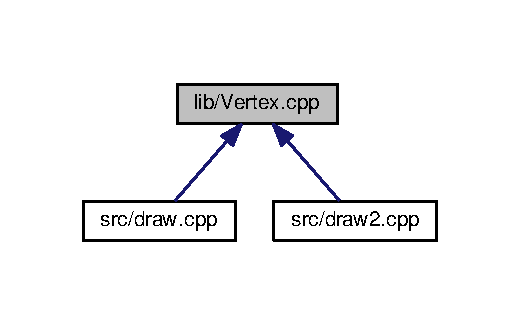
\includegraphics[width=250pt]{_vertex_8cpp__dep__incl}
\end{center}
\end{figure}
\subsection*{Classes}
\begin{DoxyCompactItemize}
\item 
struct \hyperlink{struct_vertex2_d}{Vertex2D}
\item 
struct \hyperlink{struct_point2_d}{Point2D}
\item 
struct \hyperlink{struct_vertex3_d}{Vertex3D}
\end{DoxyCompactItemize}
\subsection*{Functions}
\begin{DoxyCompactItemize}
\item 
bool \hyperlink{_vertex_8cpp_af4e16a3ca1c1611d433c534186674990}{sortfunc} (const \hyperlink{struct_vertex3_d}{Vertex3D} \&lhs, const \hyperlink{struct_vertex3_d}{Vertex3D} \&rhs)
\end{DoxyCompactItemize}


\subsection{Function Documentation}
\index{Vertex.\+cpp@{Vertex.\+cpp}!sortfunc@{sortfunc}}
\index{sortfunc@{sortfunc}!Vertex.\+cpp@{Vertex.\+cpp}}
\subsubsection[{\texorpdfstring{sortfunc(const Vertex3\+D \&lhs, const Vertex3\+D \&rhs)}{sortfunc(const Vertex3D &lhs, const Vertex3D &rhs)}}]{\setlength{\rightskip}{0pt plus 5cm}bool sortfunc (
\begin{DoxyParamCaption}
\item[{const {\bf Vertex3D} \&}]{lhs, }
\item[{const {\bf Vertex3D} \&}]{rhs}
\end{DoxyParamCaption}
)}\hypertarget{_vertex_8cpp_af4e16a3ca1c1611d433c534186674990}{}\label{_vertex_8cpp_af4e16a3ca1c1611d433c534186674990}


Definition at line 27 of file Vertex.\+cpp.


\hypertarget{_r_e_a_d_m_e_8md}{}\section{R\+E\+A\+D\+M\+E.\+md File Reference}
\label{_r_e_a_d_m_e_8md}\index{R\+E\+A\+D\+M\+E.\+md@{R\+E\+A\+D\+M\+E.\+md}}

\hypertarget{draw_8cpp}{}\section{src/draw.cpp File Reference}
\label{draw_8cpp}\index{src/draw.\+cpp@{src/draw.\+cpp}}
{\ttfamily \#include $<$math.\+h$>$}\\*
{\ttfamily \#include $<$Qt\+Core$>$}\\*
{\ttfamily \#include $<$Qt\+Gui$>$}\\*
{\ttfamily \#include $<$fstream$>$}\\*
{\ttfamily \#include $<$iostream$>$}\\*
{\ttfamily \#include \char`\"{}../lib/\+Vertex.\+cpp\char`\"{}}\\*
{\ttfamily \#include \char`\"{}Two\+To\+Three.\+cpp\char`\"{}}\\*
{\ttfamily \#include \char`\"{}Three\+To\+Two.\+cpp\char`\"{}}\\*
Include dependency graph for draw.\+cpp\+:
\nopagebreak
\begin{figure}[H]
\begin{center}
\leavevmode
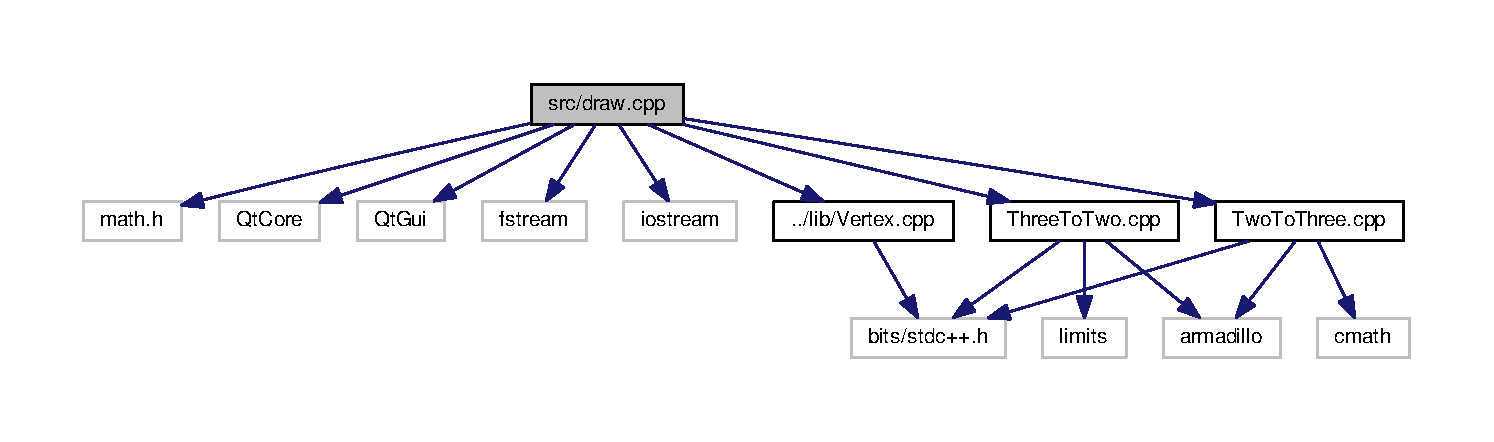
\includegraphics[width=350pt]{draw_8cpp__incl}
\end{center}
\end{figure}
\subsection*{Macros}
\begin{DoxyCompactItemize}
\item 
\#define \hyperlink{draw_8cpp_a598a3330b3c21701223ee0ca14316eca}{PI}~3.\+1415926536
\end{DoxyCompactItemize}
\subsection*{Functions}
\begin{DoxyCompactItemize}
\item 
int \hyperlink{draw_8cpp_a0ddf1224851353fc92bfbff6f499fa97}{main} (int argc, char $\ast$argv\mbox{[}$\,$\mbox{]})
\end{DoxyCompactItemize}


\subsection{Macro Definition Documentation}
\index{draw.\+cpp@{draw.\+cpp}!PI@{PI}}
\index{PI@{PI}!draw.\+cpp@{draw.\+cpp}}
\subsubsection[{\texorpdfstring{PI}{PI}}]{\setlength{\rightskip}{0pt plus 5cm}\#define PI~3.\+1415926536}\hypertarget{draw_8cpp_a598a3330b3c21701223ee0ca14316eca}{}\label{draw_8cpp_a598a3330b3c21701223ee0ca14316eca}


Definition at line 7 of file draw.\+cpp.



\subsection{Function Documentation}
\index{draw.\+cpp@{draw.\+cpp}!main@{main}}
\index{main@{main}!draw.\+cpp@{draw.\+cpp}}
\subsubsection[{\texorpdfstring{main(int argc, char $\ast$argv[])}{main(int argc, char *argv[])}}]{\setlength{\rightskip}{0pt plus 5cm}int main (
\begin{DoxyParamCaption}
\item[{int}]{argc, }
\item[{char $\ast$}]{argv\mbox{[}$\,$\mbox{]}}
\end{DoxyParamCaption}
)}\hypertarget{draw_8cpp_a0ddf1224851353fc92bfbff6f499fa97}{}\label{draw_8cpp_a0ddf1224851353fc92bfbff6f499fa97}


Definition at line 15 of file draw.\+cpp.


\hypertarget{draw2_8cpp}{}\section{src/draw2.cpp File Reference}
\label{draw2_8cpp}\index{src/draw2.\+cpp@{src/draw2.\+cpp}}
{\ttfamily \#include $<$math.\+h$>$}\\*
{\ttfamily \#include $<$fstream$>$}\\*
{\ttfamily \#include $<$iostream$>$}\\*
{\ttfamily \#include $<$G\+L/glut.\+h$>$}\\*
{\ttfamily \#include \char`\"{}../lib/\+Vertex.\+cpp\char`\"{}}\\*
{\ttfamily \#include \char`\"{}Two\+To\+Three.\+cpp\char`\"{}}\\*
{\ttfamily \#include \char`\"{}Three\+To\+Two.\+cpp\char`\"{}}\\*
Include dependency graph for draw2.\+cpp\+:
\nopagebreak
\begin{figure}[H]
\begin{center}
\leavevmode
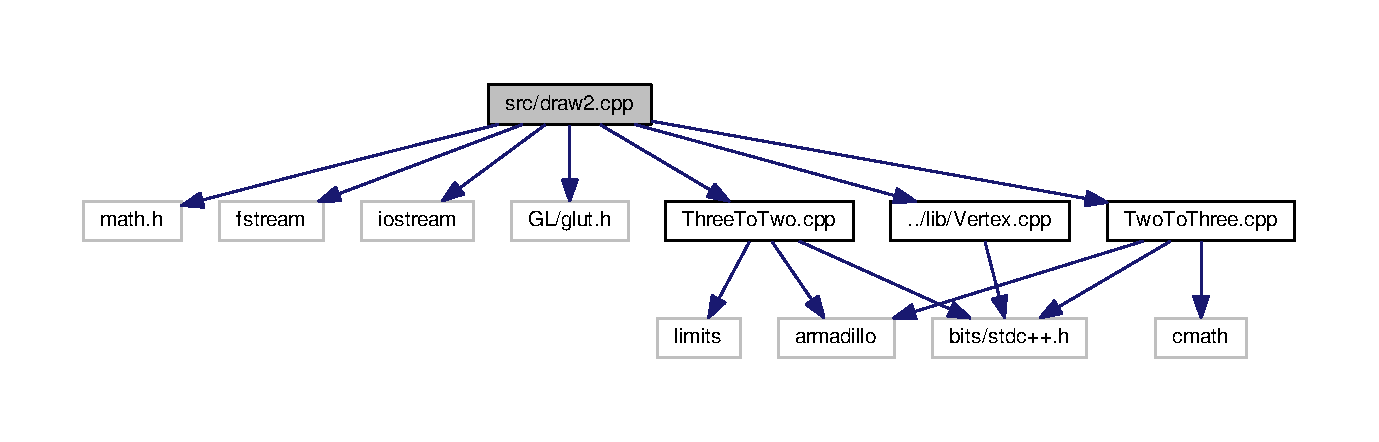
\includegraphics[width=350pt]{draw2_8cpp__incl}
\end{center}
\end{figure}
\subsection*{Macros}
\begin{DoxyCompactItemize}
\item 
\#define \hyperlink{draw2_8cpp_a598a3330b3c21701223ee0ca14316eca}{PI}~3.\+1415926536
\end{DoxyCompactItemize}
\subsection*{Functions}
\begin{DoxyCompactItemize}
\item 
void \hyperlink{draw2_8cpp_ac5c54df7ed3b930268c8d7752c101725}{update} ()
\item 
void \hyperlink{draw2_8cpp_afa20485a295d6e55ffe9d5c496d1cfa1}{idle\+\_\+fn} ()
\item 
void \hyperlink{draw2_8cpp_a1e5b20fed15743656bb6d2e6a6ea6269}{display} ()
\item 
void \hyperlink{draw2_8cpp_af4b6db54ef371626a3d23da2636a4fa0}{display1} ()
\item 
void \hyperlink{draw2_8cpp_a91cdf55e49e2c33dd11a85a178a82409}{display2} ()
\item 
void \hyperlink{draw2_8cpp_a5ae730bf155322af402f2f4b2dfcd54d}{display3} ()
\item 
void \hyperlink{draw2_8cpp_a1564b834688cdbb8c5b7614900ce833e}{Special\+\_\+\+Keys} (int key, int x, int y)
\item 
int \hyperlink{draw2_8cpp_a3c04138a5bfe5d72780bb7e82a18e627}{main} (int argc, char $\ast$$\ast$argv)
\end{DoxyCompactItemize}
\subsection*{Variables}
\begin{DoxyCompactItemize}
\item 
bool \hyperlink{draw2_8cpp_a77e49fc0956d412a05337460c7778c6d}{first} =true
\item 
int \hyperlink{draw2_8cpp_a63bd75f20c553f0d65d7bb29b3f35696}{choice}
\item 
bool \hyperlink{draw2_8cpp_a92935f074a30dac547e4bc8b6e14e31d}{choice2to3} =true
\item 
bool \hyperlink{draw2_8cpp_a13511c29978758fa77a77103770f942f}{choice3to2} =true
\item 
float \hyperlink{draw2_8cpp_a4aec1a5be9d9a4a394a2e49e9744286e}{a}
\item 
float \hyperlink{draw2_8cpp_a83fc1af92e29717b4513d121b0c72c7d}{b}
\item 
float \hyperlink{draw2_8cpp_ae78103ab33f03590e84ff7bc735629d7}{c}
\item 
float \hyperlink{draw2_8cpp_ad36c8f7a507294aa8f53bb0baf28fb24}{a1}
\item 
float \hyperlink{draw2_8cpp_a0a909289ec9fbfaa70c0e112ec9e3b15}{b1}
\item 
float \hyperlink{draw2_8cpp_a7fea4d2f6f3c31b60301494b136558af}{c1}
\item 
float \hyperlink{draw2_8cpp_a0a9ef35b787a9d8a73482c238d0177c4}{a2}
\item 
float \hyperlink{draw2_8cpp_a746bcb222044619e5a9b335d242a2a92}{b2}
\item 
float \hyperlink{draw2_8cpp_a0fe1885b4d10c978f52619ab968adadc}{c2}
\item 
float \hyperlink{draw2_8cpp_ade6a1e5a65fbbbc7812aab91226157d8}{r\+\_\+x} =0.\+0
\item 
float \hyperlink{draw2_8cpp_af623cefe51ccc3108c3cd7328a92b7fb}{r\+\_\+y} =0.\+0
\item 
string \hyperlink{draw2_8cpp_a5e321865280511fce6bc417ba1807491}{d3\+\_\+in\+File}
\item 
string \hyperlink{draw2_8cpp_a596148356aa855178797cfa8926f756b}{d2\+\_\+in\+File\+\_\+xy}
\item 
string \hyperlink{draw2_8cpp_ae5b794a1753e5d1a872eae278d803b5b}{d2\+\_\+in\+File\+\_\+yz}
\item 
string \hyperlink{draw2_8cpp_ad46a959b5a8bae75aa7829bf63b1d082}{d2\+\_\+in\+File\+\_\+zx}
\item 
int \hyperlink{draw2_8cpp_a3bf12bd6957e03ad1df6105a272ae95f}{main\+\_\+window}
\item 
int \hyperlink{draw2_8cpp_a597d6e9c3821eba36098286213f88e3b}{sub\+\_\+window1}
\item 
int \hyperlink{draw2_8cpp_a02005a3fb43ee69026c855d98a2bb47f}{sub\+\_\+window2}
\item 
int \hyperlink{draw2_8cpp_aadf72dabdff891c68d71b93c112e98f9}{sub\+\_\+window3}
\item 
int \hyperlink{draw2_8cpp_a5b714d66fd49ed892517d5e8f2f12256}{sub\+\_\+window4}
\item 
int \hyperlink{draw2_8cpp_a4365545fd48c51e8d4fa9ebb99c6a72f}{ang} =30
\end{DoxyCompactItemize}


\subsection{Macro Definition Documentation}
\index{draw2.\+cpp@{draw2.\+cpp}!PI@{PI}}
\index{PI@{PI}!draw2.\+cpp@{draw2.\+cpp}}
\subsubsection[{\texorpdfstring{PI}{PI}}]{\setlength{\rightskip}{0pt plus 5cm}\#define PI~3.\+1415926536}\hypertarget{draw2_8cpp_a598a3330b3c21701223ee0ca14316eca}{}\label{draw2_8cpp_a598a3330b3c21701223ee0ca14316eca}


Definition at line 6 of file draw2.\+cpp.



\subsection{Function Documentation}
\index{draw2.\+cpp@{draw2.\+cpp}!display@{display}}
\index{display@{display}!draw2.\+cpp@{draw2.\+cpp}}
\subsubsection[{\texorpdfstring{display()}{display()}}]{\setlength{\rightskip}{0pt plus 5cm}void display (
\begin{DoxyParamCaption}
{}
\end{DoxyParamCaption}
)}\hypertarget{draw2_8cpp_a1e5b20fed15743656bb6d2e6a6ea6269}{}\label{draw2_8cpp_a1e5b20fed15743656bb6d2e6a6ea6269}


Definition at line 314 of file draw2.\+cpp.

\index{draw2.\+cpp@{draw2.\+cpp}!display1@{display1}}
\index{display1@{display1}!draw2.\+cpp@{draw2.\+cpp}}
\subsubsection[{\texorpdfstring{display1()}{display1()}}]{\setlength{\rightskip}{0pt plus 5cm}void display1 (
\begin{DoxyParamCaption}
{}
\end{DoxyParamCaption}
)}\hypertarget{draw2_8cpp_af4b6db54ef371626a3d23da2636a4fa0}{}\label{draw2_8cpp_af4b6db54ef371626a3d23da2636a4fa0}


Definition at line 363 of file draw2.\+cpp.

\index{draw2.\+cpp@{draw2.\+cpp}!display2@{display2}}
\index{display2@{display2}!draw2.\+cpp@{draw2.\+cpp}}
\subsubsection[{\texorpdfstring{display2()}{display2()}}]{\setlength{\rightskip}{0pt plus 5cm}void display2 (
\begin{DoxyParamCaption}
{}
\end{DoxyParamCaption}
)}\hypertarget{draw2_8cpp_a91cdf55e49e2c33dd11a85a178a82409}{}\label{draw2_8cpp_a91cdf55e49e2c33dd11a85a178a82409}


Definition at line 412 of file draw2.\+cpp.

\index{draw2.\+cpp@{draw2.\+cpp}!display3@{display3}}
\index{display3@{display3}!draw2.\+cpp@{draw2.\+cpp}}
\subsubsection[{\texorpdfstring{display3()}{display3()}}]{\setlength{\rightskip}{0pt plus 5cm}void display3 (
\begin{DoxyParamCaption}
{}
\end{DoxyParamCaption}
)}\hypertarget{draw2_8cpp_a5ae730bf155322af402f2f4b2dfcd54d}{}\label{draw2_8cpp_a5ae730bf155322af402f2f4b2dfcd54d}


Definition at line 461 of file draw2.\+cpp.

\index{draw2.\+cpp@{draw2.\+cpp}!idle\+\_\+fn@{idle\+\_\+fn}}
\index{idle\+\_\+fn@{idle\+\_\+fn}!draw2.\+cpp@{draw2.\+cpp}}
\subsubsection[{\texorpdfstring{idle\+\_\+fn()}{idle_fn()}}]{\setlength{\rightskip}{0pt plus 5cm}void idle\+\_\+fn (
\begin{DoxyParamCaption}
{}
\end{DoxyParamCaption}
)}\hypertarget{draw2_8cpp_afa20485a295d6e55ffe9d5c496d1cfa1}{}\label{draw2_8cpp_afa20485a295d6e55ffe9d5c496d1cfa1}


Definition at line 298 of file draw2.\+cpp.

\index{draw2.\+cpp@{draw2.\+cpp}!main@{main}}
\index{main@{main}!draw2.\+cpp@{draw2.\+cpp}}
\subsubsection[{\texorpdfstring{main(int argc, char $\ast$$\ast$argv)}{main(int argc, char **argv)}}]{\setlength{\rightskip}{0pt plus 5cm}int main (
\begin{DoxyParamCaption}
\item[{int}]{argc, }
\item[{char $\ast$$\ast$}]{argv}
\end{DoxyParamCaption}
)}\hypertarget{draw2_8cpp_a3c04138a5bfe5d72780bb7e82a18e627}{}\label{draw2_8cpp_a3c04138a5bfe5d72780bb7e82a18e627}


Definition at line 534 of file draw2.\+cpp.

\index{draw2.\+cpp@{draw2.\+cpp}!Special\+\_\+\+Keys@{Special\+\_\+\+Keys}}
\index{Special\+\_\+\+Keys@{Special\+\_\+\+Keys}!draw2.\+cpp@{draw2.\+cpp}}
\subsubsection[{\texorpdfstring{Special\+\_\+\+Keys(int key, int x, int y)}{Special_Keys(int key, int x, int y)}}]{\setlength{\rightskip}{0pt plus 5cm}void Special\+\_\+\+Keys (
\begin{DoxyParamCaption}
\item[{int}]{key, }
\item[{int}]{x, }
\item[{int}]{y}
\end{DoxyParamCaption}
)}\hypertarget{draw2_8cpp_a1564b834688cdbb8c5b7614900ce833e}{}\label{draw2_8cpp_a1564b834688cdbb8c5b7614900ce833e}


Definition at line 509 of file draw2.\+cpp.

\index{draw2.\+cpp@{draw2.\+cpp}!update@{update}}
\index{update@{update}!draw2.\+cpp@{draw2.\+cpp}}
\subsubsection[{\texorpdfstring{update()}{update()}}]{\setlength{\rightskip}{0pt plus 5cm}void update (
\begin{DoxyParamCaption}
{}
\end{DoxyParamCaption}
)}\hypertarget{draw2_8cpp_ac5c54df7ed3b930268c8d7752c101725}{}\label{draw2_8cpp_ac5c54df7ed3b930268c8d7752c101725}


Definition at line 27 of file draw2.\+cpp.



\subsection{Variable Documentation}
\index{draw2.\+cpp@{draw2.\+cpp}!a@{a}}
\index{a@{a}!draw2.\+cpp@{draw2.\+cpp}}
\subsubsection[{\texorpdfstring{a}{a}}]{\setlength{\rightskip}{0pt plus 5cm}float a}\hypertarget{draw2_8cpp_a4aec1a5be9d9a4a394a2e49e9744286e}{}\label{draw2_8cpp_a4aec1a5be9d9a4a394a2e49e9744286e}


Definition at line 19 of file draw2.\+cpp.

\index{draw2.\+cpp@{draw2.\+cpp}!a1@{a1}}
\index{a1@{a1}!draw2.\+cpp@{draw2.\+cpp}}
\subsubsection[{\texorpdfstring{a1}{a1}}]{\setlength{\rightskip}{0pt plus 5cm}float a1}\hypertarget{draw2_8cpp_ad36c8f7a507294aa8f53bb0baf28fb24}{}\label{draw2_8cpp_ad36c8f7a507294aa8f53bb0baf28fb24}


Definition at line 20 of file draw2.\+cpp.

\index{draw2.\+cpp@{draw2.\+cpp}!a2@{a2}}
\index{a2@{a2}!draw2.\+cpp@{draw2.\+cpp}}
\subsubsection[{\texorpdfstring{a2}{a2}}]{\setlength{\rightskip}{0pt plus 5cm}float a2}\hypertarget{draw2_8cpp_a0a9ef35b787a9d8a73482c238d0177c4}{}\label{draw2_8cpp_a0a9ef35b787a9d8a73482c238d0177c4}


Definition at line 21 of file draw2.\+cpp.

\index{draw2.\+cpp@{draw2.\+cpp}!ang@{ang}}
\index{ang@{ang}!draw2.\+cpp@{draw2.\+cpp}}
\subsubsection[{\texorpdfstring{ang}{ang}}]{\setlength{\rightskip}{0pt plus 5cm}int ang =30}\hypertarget{draw2_8cpp_a4365545fd48c51e8d4fa9ebb99c6a72f}{}\label{draw2_8cpp_a4365545fd48c51e8d4fa9ebb99c6a72f}


Definition at line 292 of file draw2.\+cpp.

\index{draw2.\+cpp@{draw2.\+cpp}!b@{b}}
\index{b@{b}!draw2.\+cpp@{draw2.\+cpp}}
\subsubsection[{\texorpdfstring{b}{b}}]{\setlength{\rightskip}{0pt plus 5cm}float b}\hypertarget{draw2_8cpp_a83fc1af92e29717b4513d121b0c72c7d}{}\label{draw2_8cpp_a83fc1af92e29717b4513d121b0c72c7d}


Definition at line 19 of file draw2.\+cpp.

\index{draw2.\+cpp@{draw2.\+cpp}!b1@{b1}}
\index{b1@{b1}!draw2.\+cpp@{draw2.\+cpp}}
\subsubsection[{\texorpdfstring{b1}{b1}}]{\setlength{\rightskip}{0pt plus 5cm}float b1}\hypertarget{draw2_8cpp_a0a909289ec9fbfaa70c0e112ec9e3b15}{}\label{draw2_8cpp_a0a909289ec9fbfaa70c0e112ec9e3b15}


Definition at line 20 of file draw2.\+cpp.

\index{draw2.\+cpp@{draw2.\+cpp}!b2@{b2}}
\index{b2@{b2}!draw2.\+cpp@{draw2.\+cpp}}
\subsubsection[{\texorpdfstring{b2}{b2}}]{\setlength{\rightskip}{0pt plus 5cm}float b2}\hypertarget{draw2_8cpp_a746bcb222044619e5a9b335d242a2a92}{}\label{draw2_8cpp_a746bcb222044619e5a9b335d242a2a92}


Definition at line 21 of file draw2.\+cpp.

\index{draw2.\+cpp@{draw2.\+cpp}!c@{c}}
\index{c@{c}!draw2.\+cpp@{draw2.\+cpp}}
\subsubsection[{\texorpdfstring{c}{c}}]{\setlength{\rightskip}{0pt plus 5cm}float c}\hypertarget{draw2_8cpp_ae78103ab33f03590e84ff7bc735629d7}{}\label{draw2_8cpp_ae78103ab33f03590e84ff7bc735629d7}


Definition at line 19 of file draw2.\+cpp.

\index{draw2.\+cpp@{draw2.\+cpp}!c1@{c1}}
\index{c1@{c1}!draw2.\+cpp@{draw2.\+cpp}}
\subsubsection[{\texorpdfstring{c1}{c1}}]{\setlength{\rightskip}{0pt plus 5cm}float c1}\hypertarget{draw2_8cpp_a7fea4d2f6f3c31b60301494b136558af}{}\label{draw2_8cpp_a7fea4d2f6f3c31b60301494b136558af}


Definition at line 20 of file draw2.\+cpp.

\index{draw2.\+cpp@{draw2.\+cpp}!c2@{c2}}
\index{c2@{c2}!draw2.\+cpp@{draw2.\+cpp}}
\subsubsection[{\texorpdfstring{c2}{c2}}]{\setlength{\rightskip}{0pt plus 5cm}float c2}\hypertarget{draw2_8cpp_a0fe1885b4d10c978f52619ab968adadc}{}\label{draw2_8cpp_a0fe1885b4d10c978f52619ab968adadc}


Definition at line 21 of file draw2.\+cpp.

\index{draw2.\+cpp@{draw2.\+cpp}!choice@{choice}}
\index{choice@{choice}!draw2.\+cpp@{draw2.\+cpp}}
\subsubsection[{\texorpdfstring{choice}{choice}}]{\setlength{\rightskip}{0pt plus 5cm}int choice}\hypertarget{draw2_8cpp_a63bd75f20c553f0d65d7bb29b3f35696}{}\label{draw2_8cpp_a63bd75f20c553f0d65d7bb29b3f35696}


Definition at line 16 of file draw2.\+cpp.

\index{draw2.\+cpp@{draw2.\+cpp}!choice2to3@{choice2to3}}
\index{choice2to3@{choice2to3}!draw2.\+cpp@{draw2.\+cpp}}
\subsubsection[{\texorpdfstring{choice2to3}{choice2to3}}]{\setlength{\rightskip}{0pt plus 5cm}bool choice2to3 =true}\hypertarget{draw2_8cpp_a92935f074a30dac547e4bc8b6e14e31d}{}\label{draw2_8cpp_a92935f074a30dac547e4bc8b6e14e31d}


Definition at line 17 of file draw2.\+cpp.

\index{draw2.\+cpp@{draw2.\+cpp}!choice3to2@{choice3to2}}
\index{choice3to2@{choice3to2}!draw2.\+cpp@{draw2.\+cpp}}
\subsubsection[{\texorpdfstring{choice3to2}{choice3to2}}]{\setlength{\rightskip}{0pt plus 5cm}bool choice3to2 =true}\hypertarget{draw2_8cpp_a13511c29978758fa77a77103770f942f}{}\label{draw2_8cpp_a13511c29978758fa77a77103770f942f}


Definition at line 18 of file draw2.\+cpp.

\index{draw2.\+cpp@{draw2.\+cpp}!d2\+\_\+in\+File\+\_\+xy@{d2\+\_\+in\+File\+\_\+xy}}
\index{d2\+\_\+in\+File\+\_\+xy@{d2\+\_\+in\+File\+\_\+xy}!draw2.\+cpp@{draw2.\+cpp}}
\subsubsection[{\texorpdfstring{d2\+\_\+in\+File\+\_\+xy}{d2_inFile_xy}}]{\setlength{\rightskip}{0pt plus 5cm}string d2\+\_\+in\+File\+\_\+xy}\hypertarget{draw2_8cpp_a596148356aa855178797cfa8926f756b}{}\label{draw2_8cpp_a596148356aa855178797cfa8926f756b}


Definition at line 23 of file draw2.\+cpp.

\index{draw2.\+cpp@{draw2.\+cpp}!d2\+\_\+in\+File\+\_\+yz@{d2\+\_\+in\+File\+\_\+yz}}
\index{d2\+\_\+in\+File\+\_\+yz@{d2\+\_\+in\+File\+\_\+yz}!draw2.\+cpp@{draw2.\+cpp}}
\subsubsection[{\texorpdfstring{d2\+\_\+in\+File\+\_\+yz}{d2_inFile_yz}}]{\setlength{\rightskip}{0pt plus 5cm}string d2\+\_\+in\+File\+\_\+yz}\hypertarget{draw2_8cpp_ae5b794a1753e5d1a872eae278d803b5b}{}\label{draw2_8cpp_ae5b794a1753e5d1a872eae278d803b5b}


Definition at line 23 of file draw2.\+cpp.

\index{draw2.\+cpp@{draw2.\+cpp}!d2\+\_\+in\+File\+\_\+zx@{d2\+\_\+in\+File\+\_\+zx}}
\index{d2\+\_\+in\+File\+\_\+zx@{d2\+\_\+in\+File\+\_\+zx}!draw2.\+cpp@{draw2.\+cpp}}
\subsubsection[{\texorpdfstring{d2\+\_\+in\+File\+\_\+zx}{d2_inFile_zx}}]{\setlength{\rightskip}{0pt plus 5cm}string d2\+\_\+in\+File\+\_\+zx}\hypertarget{draw2_8cpp_ad46a959b5a8bae75aa7829bf63b1d082}{}\label{draw2_8cpp_ad46a959b5a8bae75aa7829bf63b1d082}


Definition at line 23 of file draw2.\+cpp.

\index{draw2.\+cpp@{draw2.\+cpp}!d3\+\_\+in\+File@{d3\+\_\+in\+File}}
\index{d3\+\_\+in\+File@{d3\+\_\+in\+File}!draw2.\+cpp@{draw2.\+cpp}}
\subsubsection[{\texorpdfstring{d3\+\_\+in\+File}{d3_inFile}}]{\setlength{\rightskip}{0pt plus 5cm}string d3\+\_\+in\+File}\hypertarget{draw2_8cpp_a5e321865280511fce6bc417ba1807491}{}\label{draw2_8cpp_a5e321865280511fce6bc417ba1807491}


Definition at line 23 of file draw2.\+cpp.

\index{draw2.\+cpp@{draw2.\+cpp}!first@{first}}
\index{first@{first}!draw2.\+cpp@{draw2.\+cpp}}
\subsubsection[{\texorpdfstring{first}{first}}]{\setlength{\rightskip}{0pt plus 5cm}bool first =true}\hypertarget{draw2_8cpp_a77e49fc0956d412a05337460c7778c6d}{}\label{draw2_8cpp_a77e49fc0956d412a05337460c7778c6d}


Definition at line 15 of file draw2.\+cpp.

\index{draw2.\+cpp@{draw2.\+cpp}!main\+\_\+window@{main\+\_\+window}}
\index{main\+\_\+window@{main\+\_\+window}!draw2.\+cpp@{draw2.\+cpp}}
\subsubsection[{\texorpdfstring{main\+\_\+window}{main_window}}]{\setlength{\rightskip}{0pt plus 5cm}int main\+\_\+window}\hypertarget{draw2_8cpp_a3bf12bd6957e03ad1df6105a272ae95f}{}\label{draw2_8cpp_a3bf12bd6957e03ad1df6105a272ae95f}


Definition at line 25 of file draw2.\+cpp.

\index{draw2.\+cpp@{draw2.\+cpp}!r\+\_\+x@{r\+\_\+x}}
\index{r\+\_\+x@{r\+\_\+x}!draw2.\+cpp@{draw2.\+cpp}}
\subsubsection[{\texorpdfstring{r\+\_\+x}{r_x}}]{\setlength{\rightskip}{0pt plus 5cm}float r\+\_\+x =0.\+0}\hypertarget{draw2_8cpp_ade6a1e5a65fbbbc7812aab91226157d8}{}\label{draw2_8cpp_ade6a1e5a65fbbbc7812aab91226157d8}


Definition at line 22 of file draw2.\+cpp.

\index{draw2.\+cpp@{draw2.\+cpp}!r\+\_\+y@{r\+\_\+y}}
\index{r\+\_\+y@{r\+\_\+y}!draw2.\+cpp@{draw2.\+cpp}}
\subsubsection[{\texorpdfstring{r\+\_\+y}{r_y}}]{\setlength{\rightskip}{0pt plus 5cm}float r\+\_\+y =0.\+0}\hypertarget{draw2_8cpp_af623cefe51ccc3108c3cd7328a92b7fb}{}\label{draw2_8cpp_af623cefe51ccc3108c3cd7328a92b7fb}


Definition at line 22 of file draw2.\+cpp.

\index{draw2.\+cpp@{draw2.\+cpp}!sub\+\_\+window1@{sub\+\_\+window1}}
\index{sub\+\_\+window1@{sub\+\_\+window1}!draw2.\+cpp@{draw2.\+cpp}}
\subsubsection[{\texorpdfstring{sub\+\_\+window1}{sub_window1}}]{\setlength{\rightskip}{0pt plus 5cm}int sub\+\_\+window1}\hypertarget{draw2_8cpp_a597d6e9c3821eba36098286213f88e3b}{}\label{draw2_8cpp_a597d6e9c3821eba36098286213f88e3b}


Definition at line 25 of file draw2.\+cpp.

\index{draw2.\+cpp@{draw2.\+cpp}!sub\+\_\+window2@{sub\+\_\+window2}}
\index{sub\+\_\+window2@{sub\+\_\+window2}!draw2.\+cpp@{draw2.\+cpp}}
\subsubsection[{\texorpdfstring{sub\+\_\+window2}{sub_window2}}]{\setlength{\rightskip}{0pt plus 5cm}int sub\+\_\+window2}\hypertarget{draw2_8cpp_a02005a3fb43ee69026c855d98a2bb47f}{}\label{draw2_8cpp_a02005a3fb43ee69026c855d98a2bb47f}


Definition at line 25 of file draw2.\+cpp.

\index{draw2.\+cpp@{draw2.\+cpp}!sub\+\_\+window3@{sub\+\_\+window3}}
\index{sub\+\_\+window3@{sub\+\_\+window3}!draw2.\+cpp@{draw2.\+cpp}}
\subsubsection[{\texorpdfstring{sub\+\_\+window3}{sub_window3}}]{\setlength{\rightskip}{0pt plus 5cm}int sub\+\_\+window3}\hypertarget{draw2_8cpp_aadf72dabdff891c68d71b93c112e98f9}{}\label{draw2_8cpp_aadf72dabdff891c68d71b93c112e98f9}


Definition at line 25 of file draw2.\+cpp.

\index{draw2.\+cpp@{draw2.\+cpp}!sub\+\_\+window4@{sub\+\_\+window4}}
\index{sub\+\_\+window4@{sub\+\_\+window4}!draw2.\+cpp@{draw2.\+cpp}}
\subsubsection[{\texorpdfstring{sub\+\_\+window4}{sub_window4}}]{\setlength{\rightskip}{0pt plus 5cm}int sub\+\_\+window4}\hypertarget{draw2_8cpp_a5b714d66fd49ed892517d5e8f2f12256}{}\label{draw2_8cpp_a5b714d66fd49ed892517d5e8f2f12256}


Definition at line 25 of file draw2.\+cpp.


\hypertarget{main_8cpp}{}\section{src/main.cpp File Reference}
\label{main_8cpp}\index{src/main.\+cpp@{src/main.\+cpp}}
{\ttfamily \#include $<$iostream$>$}\\*
{\ttfamily \#include $<$cstdlib$>$}\\*
Include dependency graph for main.\+cpp\+:
\nopagebreak
\begin{figure}[H]
\begin{center}
\leavevmode
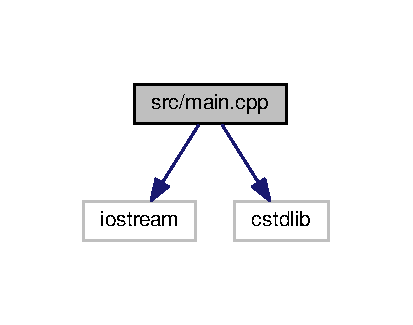
\includegraphics[width=198pt]{main_8cpp__incl}
\end{center}
\end{figure}
\subsection*{Functions}
\begin{DoxyCompactItemize}
\item 
int \hyperlink{main_8cpp_ae66f6b31b5ad750f1fe042a706a4e3d4}{main} ()
\end{DoxyCompactItemize}


\subsection{Function Documentation}
\index{main.\+cpp@{main.\+cpp}!main@{main}}
\index{main@{main}!main.\+cpp@{main.\+cpp}}
\subsubsection[{\texorpdfstring{main()}{main()}}]{\setlength{\rightskip}{0pt plus 5cm}int main (
\begin{DoxyParamCaption}
{}
\end{DoxyParamCaption}
)}\hypertarget{main_8cpp_ae66f6b31b5ad750f1fe042a706a4e3d4}{}\label{main_8cpp_ae66f6b31b5ad750f1fe042a706a4e3d4}


Definition at line 6 of file main.\+cpp.


\hypertarget{_three_to_two_8cpp}{}\section{src/\+Three\+To\+Two.cpp File Reference}
\label{_three_to_two_8cpp}\index{src/\+Three\+To\+Two.\+cpp@{src/\+Three\+To\+Two.\+cpp}}
{\ttfamily \#include $<$bits/stdc++.\+h$>$}\\*
{\ttfamily \#include $<$armadillo$>$}\\*
{\ttfamily \#include $<$limits$>$}\\*
Include dependency graph for Three\+To\+Two.\+cpp\+:
\nopagebreak
\begin{figure}[H]
\begin{center}
\leavevmode
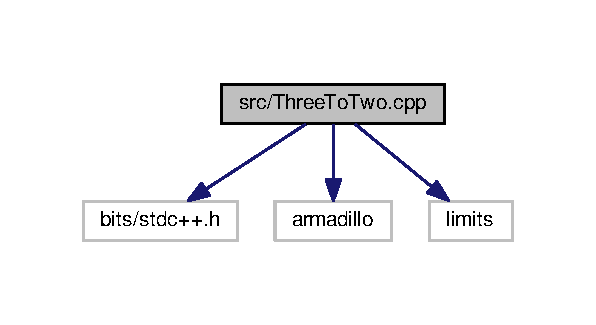
\includegraphics[width=286pt]{_three_to_two_8cpp__incl}
\end{center}
\end{figure}
This graph shows which files directly or indirectly include this file\+:
\nopagebreak
\begin{figure}[H]
\begin{center}
\leavevmode
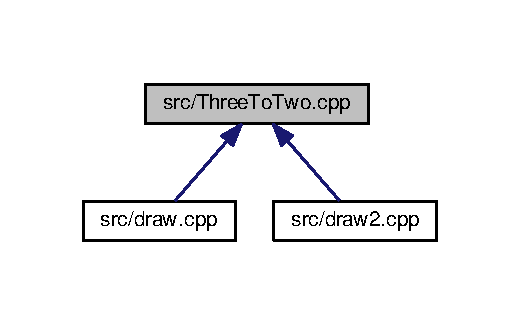
\includegraphics[width=250pt]{_three_to_two_8cpp__dep__incl}
\end{center}
\end{figure}
\subsection*{Classes}
\begin{DoxyCompactItemize}
\item 
class \hyperlink{class_three___to___two}{Three\+\_\+\+To\+\_\+\+Two}
\end{DoxyCompactItemize}

\hypertarget{_two_to_three_8cpp}{}\section{src/\+Two\+To\+Three.cpp File Reference}
\label{_two_to_three_8cpp}\index{src/\+Two\+To\+Three.\+cpp@{src/\+Two\+To\+Three.\+cpp}}
{\ttfamily \#include $<$bits/stdc++.\+h$>$}\\*
{\ttfamily \#include $<$armadillo$>$}\\*
{\ttfamily \#include $<$cmath$>$}\\*
Include dependency graph for Two\+To\+Three.\+cpp\+:
\nopagebreak
\begin{figure}[H]
\begin{center}
\leavevmode
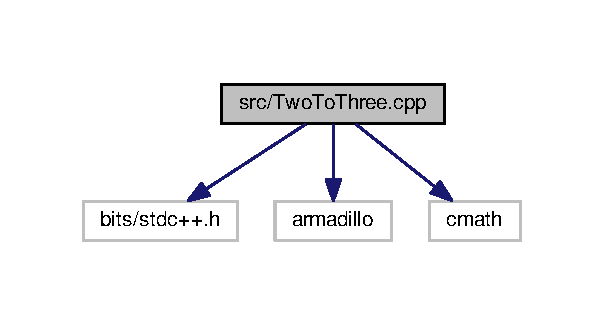
\includegraphics[width=290pt]{_two_to_three_8cpp__incl}
\end{center}
\end{figure}
This graph shows which files directly or indirectly include this file\+:
\nopagebreak
\begin{figure}[H]
\begin{center}
\leavevmode
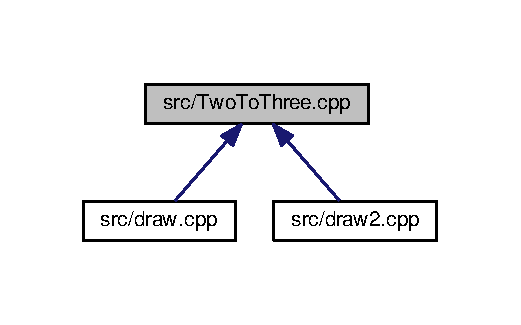
\includegraphics[width=250pt]{_two_to_three_8cpp__dep__incl}
\end{center}
\end{figure}
\subsection*{Classes}
\begin{DoxyCompactItemize}
\item 
class \hyperlink{class_two___to___three}{Two\+\_\+\+To\+\_\+\+Three}
\end{DoxyCompactItemize}

%--- End generated contents ---

% Index
\backmatter
\newpage
\phantomsection
\clearemptydoublepage
\addcontentsline{toc}{chapter}{Index}
\printindex

\end{document}
